%%%%%%%%%%%%%%%%%%%%%%%%%%%%%%%%%%%%%%%%%%%%%%%%%%%%%%%%%%%%%%%%%%%%%%%%%%%%
%% Trim Size: 9.75in x 6.5in
%% Text Area: 8in (include Runningheads) x 5in
%% ws-ijsc.tex     14-2-07
%% Tex file to use with ws-ijsc.cls written in Latex2E. 
%% The content, structure, format and layout of this style file is the 
%% property of World Scientific Publishing Co. Pte. Ltd. 
%% Copyright 1995, 2002 by World Scientific Publishing Co. 
%% All rights are reserved.
%%%%%%%%%%%%%%%%%%%%%%%%%%%%%%%%%%%%%%%%%%%%%%%%%%%%%%%%%%%%%%%%%%%%%%%%%%%%
%%

\documentclass{ws-ijsc}

% correct bad hyphenation here
\hyphenation{op-tical net-works semi-conduc-tor}







% allows for temporary adjustment of side margins
\usepackage{chngpage}

% just makes the table prettier (see \toprule, \bottomrule, etc. commands below)
\usepackage{booktabs}

\usepackage[utf8]{inputenc}
%\usepackage[font=small,skip=0pt]{caption}

% footnotes
\usepackage{scrextend}

% colors
\usepackage[usenames, dvipsnames]{color}

% underline
\usepackage{tikz}
\newcommand{\udensdot}[1]{%
    \tikz[baseline=(todotted.base)]{
        \node[inner sep=1pt,outer sep=0pt] (todotted) {#1};
        \draw[densely dotted] (todotted.south west) -- (todotted.south east);
    }%
}%

\newcommand{\uloosdot}[1]{%
    \tikz[baseline=(todotted.base)]{
        \node[inner sep=1pt,outer sep=0pt] (todotted) {#1};
        \draw[loosely dotted] (todotted.south west) -- (todotted.south east);
    }%
}%

\newcommand{\udash}[1]{%
    \tikz[baseline=(todotted.base)]{
        \node[inner sep=1pt,outer sep=0pt] (todotted) {#1};
        \draw[dashed] (todotted.south west) -- (todotted.south east);
    }%
}%

\newcommand{\udensdash}[1]{%
    \tikz[baseline=(todotted.base)]{
        \node[inner sep=1pt,outer sep=0pt] (todotted) {#1};
        \draw[densely dashed] (todotted.south west) -- (todotted.south east);
    }%
}%

\newcommand{\uloosdash}[1]{%
    \tikz[baseline=(todotted.base)]{
        \node[inner sep=1pt,outer sep=0pt] (todotted) {#1};
        \draw[loosely dashed] (todotted.south west) -- (todotted.south east);
    }%
}%

% URL handling
\usepackage{url}
\urlstyle{same}

%\usepackage{makeidx}  % allows for indexgeneration

%\usepackage{amsmath}
\usepackage{amsmath, amssymb}
\usepackage{mathabx}
\usepackage{caption} 
\captionsetup[table]{skip=10pt}

% monospace within text
\newcommand{\ms}[1]{\texttt{#1}}

% examples
\usepackage{fancyvrb}
\DefineVerbatimEnvironment{ex}{Verbatim}{numbers=left,numbersep=2mm,frame=single,fontsize=\scriptsize}

\usepackage{xspace}
% Einfache und doppelte Anfuehrungszeichen
\newcommand{\qs}{``} 
\newcommand{\qe}{''\xspace} 
\newcommand{\sqs}{`} 
\newcommand{\sqe}{'\xspace} 

% checkmark
\usepackage{tikz}
\def\checkmark{\tikz\fill[scale=0.4](0,.35) -- (.25,0) -- (1,.7) -- (.25,.15) -- cycle;} 

% Xs
\usepackage{pifont}

% Tabellenabstände kleiner
\setlength{\intextsep}{10pt} % Vertical space above & below [h] floats
\setlength{\textfloatsep}{10pt} % Vertical space below (above) [t] ([b]) floats
% \setlength{\abovecaptionskip}{0pt}
% \setlength{\belowcaptionskip}{0pt}

\usepackage{tabularx}
\newcommand{\hr}{\hline\noalign{\smallskip}} % für die horizontalen linien in tabellen

% Todos
\usepackage[colorinlistoftodos]{todonotes}
\newcommand{\ke}[1]{\todo[size=\small, color=red!40]{\textbf{Kai:} #1}}
\newcommand{\tb}[1]{\todo[size=\small, color=green!40]{\textbf{Thomas:} #1}}
\newcommand{\bz}[1]{\todo[size=\small, color=blue!40]{\textbf{Ben:} #1}}

\newenvironment{table-1cols}{
  \scriptsize
  \sffamily
  \vspace{0.3cm}
  \begin{tabular}{l}
  \hline
  \textbf{Requirements} \\
  \hline

}{
  \hline
  \end{tabular}
  \linebreak
}

\newenvironment{table-2cols}{
  \scriptsize
  \sffamily
  \vspace{0.3cm}
  \begin{tabular}{l|l}
  \hline
  \textbf{Requirements} & \textbf{Covering DSCLs} \\
  \hline

}{
  \hline
  \end{tabular}
  \linebreak
}

\newenvironment{complexity}{
  %\scriptsize
  %\sffamily
  %\vspace{0.3cm}
  \begin{tabular}{l|l}
  \hline
  \textbf{Complexity Class} & \textbf{Complexity} \\
  \hline

}{
  \hline
  \end{tabular}
  \linebreak
}

\newenvironment{DL}{
  %\scriptsize
  %\sffamily
  \small
  \vspace{0cm}
	\begin{center}
  \begin{tabular}{c l}

}{
  \end{tabular}
	\end{center}
}


\newenvironment{evaluation}{
  %\scriptsize
  %\sffamily
  %\vspace{0.3cm}
  \begin{tabular}{l|c|c|c|c|c|c}
  \hline
  \textbf{Constraint Class} & \textbf{DSP} & \textbf{OWL2-DL} & \textbf{OWL2-QL} & \textbf{ReSh} & \textbf{ShEx} & \textbf{SPIN} \\
  \hline

}{
  \hline
  \end{tabular}
  \linebreak
}

\newenvironment{constraint-languages-complexity}{
  %\scriptsize
  %\sffamily
  %\vspace{0.3cm}
  \begin{tabular}{l|c|c|c|c|c|c}
  \hline
  \textbf{Complexity Class} & \textbf{DSP} & \textbf{OWL2-DL} & \textbf{OWL2-QL} & \textbf{ReSh} & \textbf{ShEx} & \textbf{SPIN} \\
  \hline

}{
  \hline
  \end{tabular}
  \linebreak
}

\newenvironment{user-fiendliness}{
  %\scriptsize
  %\sffamily
  %\vspace{0.3cm}
  \begin{tabular}{l|c|c|c|c|c}
  \hline
  \textbf{criterion} & \textbf{DSP} & \textbf{OWL2} & \textbf{ReSh} & \textbf{ShEx} & \textbf{SPIN} \\
  \hline

}{
  \hline
  \end{tabular}
  \linebreak
}

\setcounter{secnumdepth}{5}

% tables
\usepackage{array,graphicx}
\usepackage{booktabs}
\usepackage{pifont}
\newcommand*\rot{\rotatebox{90}}
\newcommand*\OK{\ding{51}}
\usepackage{booktabs}
\newcommand*\ON[0]{$\surd$}

\usepackage{tablefootnote}

\usepackage{float}

\usepackage{ntheorem}
\newtheorem{hyp}{Finding}

\makeatletter
\newcounter{subhyp} 
\let\savedc@hyp\c@hyp
\newenvironment{subhyp}
 {%
  \setcounter{subhyp}{0}%
  \stepcounter{hyp}%
  \edef\saved@hyp{\thehyp}% Save the current value of hyp
  \let\c@hyp\c@subhyp     % Now hyp is subhyp
  \renewcommand{\thehyp}{\saved@hyp\alph{hyp}}%
 }
 {}
\newcommand{\normhyp}{%
  \let\c@hyp\savedc@hyp % revert to the old one
  \renewcommand\thehyp{\arabic{hyp}}%
} 
\makeatother

\usepackage{multirow}

\begin{document}

\markboth{Thomas Hartmann, Benjamin Zapilko, Joachim Wackerow, Kai Eckert}
{Directing the Development of Constraint Languages}

%%%%%%%%%%%%%%%%%%%%% Publisher's Area please ignore %%%%%%%%%%%%%%%
%
\catchline{}{}{}{}{}
%
%%%%%%%%%%%%%%%%%%%%%%%%%%%%%%%%%%%%%%%%%%%%%%%%%%%%%%%%%%%%%%%%%%%%

\title{DIRECTING THE DEVELOPMENT OF CONSTRAINT LANGUAGES BY CHECKING CONSTRAINTS ON RDF DATA}

\author{THOMAS HARTMANN}

\address{Monitoring Society and Social Change, GESIS - Leibniz Institute for the Social Sciences, \\ Square B2 1,
Mannheim, 68159, Germany\,\\
\email{thomas.hartmann@gesis.org}
\http{www.gesis.org}
}

\author{BENJAMIN ZAPILKO}

\address{Knowledge Technologies for the Social Sciences, GESIS - Leibniz Institute for the Social Sciences, Unter Sachsenhausen 6-8\\
Cologne, 50667, Germany\,\\
\email{benjamin.zapilko@gesis.org}
}

\author{JOACHIM WACKEROW}

\address{Monitoring Society and Social Change, GESIS - Leibniz Institute for the Social Sciences, \\ Square B2 1,
Mannheim, 68159, Germany\,\\
\email{joachim.wackerow@gesis.org}
}

\author{KAI ECKERT}

\address{WISS Research Group, Faculty of Information and Communication, Stuttgart Media University, \\ Nobelstraße 10,
Stuttgart, 70569, Germany\,\\
\email{eckert@hdm-stuttgart.de}
}

\maketitle

\begin{history}
\received{(Day Month Year)}
\revised{(Day Month Year)}
\accepted{(Day Month Year)}
%\comby{(xxxxxxxxxx)}
\end{history}

\begin{abstract}
For research institutes, data libraries, and data archives,
validating RDF data according to predefined constraints is a much sought-after feature, 
particularly as this is taken for granted in the XML world.
Based on our work in two international working groups on RDF validation and jointly identified requirements to formulate constraints and validate RDF data, we have published 81 types of constraints that are required by various stakeholders for data applications.

In this paper, we evaluate the usability of identified constraint types for assessing RDF data quality by (1) collecting and classifying 115 constraints on vocabularies commonly used in the social, behavioral, and economic sciences, either from the vocabularies themselves or from domain experts, and (2) validating 15,694 data sets (4.26 billion triples) of research data against these constraints. We classify each constraint according to (1) the severity of occurring violations and (2) based on which types of constraint languages are able to express its constraint type. Based on the large-scale evaluation, we formulate several findings to direct the further development of constraint languages. 
\end{abstract}

\keywords{RDF Data Validation; RDF Data Quality; Constraint Languages; Semantic Web; Linked Data; RDF.}

\section{Introduction}
% no \IEEEPARstart


%\hfill mds
 
%\hfill January 11, 2007

%%% Findings aus dem Abstract
%%% (1) for well-established vocabularies, the explicitly defined constraints are almost completely satisfied which demonstrates that constraint formulation in general works. (2) A significant amount of 47\% of the violations refer to complex constraints that are not easily expressible in existing languages which confirms the necessity to provide suitable constraint languages.  (3) The percentage of severe constraint violations is very low, compared to about 2/3 of warning violations and 1/3 of informational violations, which implies that proper constraint languages can significantly improve the data quality beyond fundamental requirements.

For constraint formulation and RDF data validation, several languages exist or are currently developed. \emph{Shape Expressions (ShEx)}, \emph{Resource Shapes (ReSh)}, \emph{Description Set Profiles (DSP)}, the \emph{Web Ontology Language (OWL)}, the \emph{SPARQL Inferencing Notation (SPIN)}, and the \emph{SPARQL Query Language for RDF} are the six most promising and widely used constraint languages. OWL is used as a constraint language under the closed-world and unique name assumptions. With its direct support of validation via SPARQL, SPIN is very popular and certainly plays an important role for future developments in this field. It is particularly interesting as a means to validate arbitrary constraint languages by mapping them to SPARQL \cite{BoschEckert2014-2}. In addition, the W3C currently develops the \emph{Shapes Constraint Language (SHACL)}, an RDF vocabulary for describing RDF graph structures. Yet, there is no clear favorite and none of the languages is able to meet all requirements raised by data practitioners. This is the reason why further research on RDF validation and the development of constraint languages is needed.

In 2013, the W3C organized the RDF Validation Workshop,
where experts from industry, government, and academia discussed first use cases for constraint formulation and RDF data validation.
In 2014, two working groups on RDF validation have been established to develop a language to express constraints on RDF data: 
the \emph{W3C RDF Data Shapes Working Group} and the \emph{DCMI RDF Application Profiles Task Group} which among others bundles the requirements of data institutions of the cultural heritage sector and the \emph{social, behavioral, and economic (SBE)} sciences and represents them in the W3C working group. 

Within the DCMI working group, a collaboratively curated database of RDF validation requirements, online available at \url{http://purl.org/net/rdf-validation}, has been created which contains the findings of the working groups based on various case studies provided by various data institutions \cite{BoschEckert2014}. 
The database connects requirements to use cases, case studies, and solutions and forms the basis of this paper. 
Based on our work in these working groups and jointly identified requirements to formulate constraints and validate RDF data, we have published 81 types of constraints; each of them corresponding to a requirement in the database.

In this paper, we collected 115 constraints for three vocabularies commonly used in the SBE domain (see Sec. \ref{sbe-vocabularies}), either from the vocabularies themselves or from several domain and data experts, in order to gain a better understanding about the role of certain constraint types for assessing data quality. 
We let the experts classify the constraints according to the severity of their violation. Furthermore, we classified each constraint type based on whether it is expressible by RDFS/OWL, common high-level constraint languages, or only by plain SPARQL (see Sec.~\ref{classification}).

As we do not want to base our conclusions on the evaluation of vocabularies and constraint definitions alone, we conducted a large-scale experiment.
For all these 115 constraints on the vocabularies DDI-RDF, QB, and SKOS, we evaluated the data quality of 15,694 data sets (4.26 billion triples) of SBE research data, obtained from 33 SPARQL endpoints.
%evaluated the data quality of 15,694 data sets (4.26 billion triples) of research data for the social, behavioral, and economic (SBE) sciences obtained from 33 SPARQL endpoints.
Based on the evaluation results,
we formulate several findings to direct the further development of constraint languages.
To make valid general statements for all vocabularies, however,
these findings still have to be verified or falsified
by evaluating the quality of data represented by more than three vocabularies (see Sec. \ref{evaluation}).
%The \textbf{contribution} of this paper is the development of a system 
%\begin{enumerate}
	%\item to classify RDF constraints (according to their severity levels) to evaluate the quality of metadata and data which may be represented by any vocabulary and 
	%\item to classify RDF constraint types (according to their complexity) which in most cases correspond to RDF validation requirements\footnote{For simplicity reasons, we use the terms \emph{constraint types} and \emph{constraints} instead of \emph{RDF constraint types} and \emph{RDF constraints} in the rest of the paper} (sections \ref{classification} - \ref{SPARQL-based-constraint-types}).
%\end{enumerate}
%By defining a huge amount of constraints of the majority of the constraint types,   
%we apply the developed classification system to several and different vocabularies from the SBE domain to represent both metadata and data and therefore prove its generality.
%A complex and complete real world running example from the SBE domain serves to prove the claim that the developed classification system perfectly applies for diverse vocabularies.
%%, i.e., that it does not matter which vocabularies are used to represent (meta)data and for which domains constraints are defined.
%We describe why RDF validation is important for the SBE community (section \ref{motivation}), 
%how data in tabular format and metadata on unit-record data sets, aggregated data sets, and thesauri are represented in RDF, 
%how therefore reused vocabularies are interrelated (section \ref{rdf-representation}),
%and how SBE (meta)data is validated against constraints of different constraint types (sections \ref{classification} - \ref{SPARQL-based-constraint-types}).
%We evaluated the (meta)data quality of large real world data sets (more than 4.2 billion triples and 15 thousand data sets) from the SBE domain represented by multiple vocabularies to get an understanding 
%(1) which sets of constraint types (on different levels of complexity) and 
%(2) which sets of constraints (associated with particular severity levels) encompass the constraints causing the most/fewest constraint violations (see section \ref{evaluation}).

In Sec. \ref{implementation}, we delineate how we implemented our validation environment which can directly be used to validate RDF data against constraints expressed in any RDF-based constraint language and extracted from or defined for any RDF vocabulary.

In this paper, we discuss constraints on RDF data in general. Note that the data represented in RDF can be data in the sense of the SBE sciences, but also metadata about published or unpublished data. We generally refer to both simply as RDF data and only distinguish between data and metadata in the data set descriptions. 
%and in the case that it matters for the purpose of this paper.

%We propose an extensible metric to measure the continuum of severity levels to indicate how serious the violation of given constraints is.
%Constraints are instantiated from constraint types in order to validate both metadata and data represented by any vocabulary. 
%As constraint types are used to define constraints on (meta)data expressed by any vocabulary, the proposed constraint classification can be applied generically, i.e. vocabulary-independent. 

%\section{Running Example}
%\label{running-example}
\section{Common Vocabularies in the SBE Sciences}
\label{sbe-vocabularies}

We took all well-established and newly developed SBE vocabularies into account and defined constraints for three vocabularies commonly used in the SBE sciences. We analyzed actual data according to constraint violations, as for these vocabularies large data sets have already been published.

%-----
%
%The data most often used in research within SBE sciences is \emph{unit-record data}, i.e., data collected about individuals, businesses, and households, in form of responses to studies or taken from administrative registers such as hospital records or registers of births and deaths. A \emph{study} represents the process by which a data set was generated or collected. The range of unit-record data is very broad - including census, education, health data and business, social, and labor force surveys. This type of research data is held within data archives or data libraries after it has been collected, so that it may be reused by future researchers. By its nature, unit-record data is highly confidential and access is often only permitted for qualified researchers who must apply for access. Researchers typically represent their results as aggregated data in form of multi-dimensional tables with only a few columns: so-called \emph{variables} such as \emph{sex} or \emph{age}. Aggregated data, which answers particular research questions, is derived from unit-record data by statistics on groups or aggregates such as frequencies and arithmetic means. The purpose of publicly available aggregated data is to get a first overview and to gain an interest in further analyses of the underlying unit-record data. For more detailed analyses, researchers refer to unit-record data including additional variables needed to answer subsequent research questions. 
%
%\emph{Formal childcare} is an example of an aggregated variable which captures the measured availability of childcare services in percent over the population in European Union member states by 
%the dimensions \emph{year}, \emph{duration}, \emph{age} of the child, and \emph{country}.
%Variables are constructed out of values (of one or multiple datatypes) and/or code lists.
%The variable \emph{age}, e.g., may be represented by values of the datatype \emph{xsd:nonNegativeInteger} or by a code list of age clusters (e.g., '0 to 10' and '11 to 20'). 
%The \emph{RDF Data Cube Vocabulary (QB)}\footnote{http://www.w3.org/TR/vocab-data-cube/} is a W3C recommendation for representing \emph{data cubes}, i.e., multi-dimensional aggregated data, in RDF \cite{Cyganiak2010}. 
%%QB represents metadata on multi-dimensional aggregate data in two files: a \emph{qb:DataSet} and a \emph{qb:DataStructureDefinition}.
%A \emph{qb:DataStructureDefinition} contains metadata of the data collection.
%The variable \emph{formal childcare} is modeled as \emph{qb:measure}, since it stands for what has been measured in the data collection.
%\emph{Year}, \emph{duration}, \emph{age}, and \emph{country} are \emph{qb:dimensions}.
%Data values, i.e., the availability of childcare services in percent over the population, are collected in a \emph{qb:DataSet}. 
%Each data value is represented inside a \emph{qb:Observation} which contains values for each dimension. 
%%(e.g., the year in which \emph{formal childcare} has been determined).
%%\ke{Wieso springt das von einer sehr knappen Einführung direkt zu konkreten (beliebigen?) Variablen? Ich möchte wissen, wofür QB benutzt wird und gerne ein konkretes %Beispiel sehen, um mir einen Data Cube vorstellen zu können.}\tb{hmm, ich halte das beispiel für ein knappes und verständliches beipsiel wie eine tabelle in qb dargestellt wird / es ist auch der link enthalten zu der tabelle von eurostat}
%
%For more detailed analyses we refer to the underlying unit-record data. The aggregated variable \emph{formal childcare} is calculated on the basis of six unit-record variables (i.a., \emph{Education at pre-school}) for which detailed metadata is given (i.a., code lists) enabling researchers to replicate the results shown in aggregated data tables.
%\emph{DDI-RDF} is used to represent metadata on unit-record data in RDF.
%%The series (\emph{DDI-RDF:StudyGroup}) \emph{EU-SILC} contains one study (\emph{DDI-RDF:Study}) for each year (\emph{dcterms:temporal}) of data collection.   
%%\emph{dcterms:spatial} points to the countries for which the data has been collected.
%The study (\emph{disco:Study}) for which the unit-record data has been collected 
%%\emph{EU-SILC 2011} 
%contains eight data sets (\emph{disco:LogicalDataSet})
%including variables (\emph{disco:Variable}) like the six ones needed to calculate the variable \emph{formal childcare}.
%%Metadata on unit-record data enables researchers to investigate further research questions based on promising findings of other researchers in form of aggregated data.
%%One common research question is ,e.g., the comparison of variables like 
%%\emph{formal childcare} between countries, for which the variable is collected within the context of an individual study, and other European or non European countries (e.g. OSCE).
%
%The \emph{Simple Knowledge Organization System (SKOS)} is reused to a large extend to build SBE vocabularies.
%The codes of the variable \emph{Education at pre-school} are modeled as \emph{skos:Concepts} and 
%a \emph{skos:OrderedCollection} organizes them in a particular order within a \emph{skos:memberList}.
%A variable may be associated with a theoretical concept (\emph{skos:Concept}) and \emph{skos:narrower} builds the hierarchy of theoretical concepts within a \emph{skos:ConceptScheme} of a study.
%The variable \emph{Education at pre-school} is assigned to the theoretical concept \emph{Child Care} which is a narrower concept of the top concept \emph{Education}.
%Controlled vocabularies (\emph{skos:ConceptScheme}), serving as extension and reuse mechanism,
%organize types (\emph{skos:Concept}) of descriptive statistics (\emph{disco:SummaryStatistics}) like minimum, maximum, and arithmetic mean.

The data most often used in research within SBE sciences is \emph{unit-record data}, i.e., data collected about individuals, businesses, and households, in form of responses to studies or taken from administrative registers such as hospital records, registers of births and deaths. A \emph{study} represents the process by which a data set was generated or collected. The range of unit-record data is very broad - including census, education, and health data and business, social, and labor force surveys. This type of research data is held within data archives or data libraries after it has been collected, so that it may be reused by future researchers. 

\subsection{Vocabularies for representing multi-dimensional aggregated data and its metadata}

By its nature, unit-record data is highly confidential and access is often only permitted for qualified researchers who must apply for access. 
Researchers typically represent their results as aggregated data in form of multi-dimensional tables with only a few columns, so-called \emph{variables} such as \emph{sex} or \emph{age}.
Aggregated data, which answers particular research questions, is derived from unit-record data by statistics on groups or aggregates such as frequencies and arithmetic means.
The purpose of publicly available aggregated data is to get a first overview and to gain an interest in further analyses on the underlying unit-record data.
Aggregated data is published in form of CSV files,
allowing to perform calculations on the data.

For more detailed analyses, researchers refer to unit-record data including additional variables needed to answer subsequent research questions
like the comparison of studies between countries.
\emph{Eurostat}, the statistical office of the European Union, provides research findings in form of aggregated data (downloadable as CSV files) and its metadata on European level that enable comparisons between countries.
\emph{Formal childcare} is an example of an aggregated variable which captures the measured availability of childcare services in percent over the population in European Union member states by 
the dimensions \emph{year}, \emph{duration}, \emph{age} of the child, and \emph{country}.
Variables are constructed out of values (of one or multiple datatypes) and/or code lists.
The variable \emph{age}, e.g., may be represented by values of the datatype \emph{xsd:nonNegativeInteger} or by a code list of age clusters (e.g., '0 to 10' and '11 to 20'). 

A representative RDF validation case study within the SBE sciences is to ensure correctness when comparing variables between data collections of different countries.
Several vocabulary-specific constraints on RDF data are checked for each data collection
in order to determine if variables measuring \emph{age} 
- collected for different countries (\emph{$age_{DE}$}, \emph{$age_{UK}$}) - 
are comparable:
(1) variable definitions must be available, 
(2) for each code a human-readable label has to be specified,
(3) code lists must be structured properly, and
(4) code lists must either be identical or at least similar.
If a researcher only wants to get a first overview on the comparability of variables (use case 1), 
covering the first three constraints may be sufficient,
i.e., the violation of the first three constraints is more serious than the violation of the last constraint.
If the intention of the researcher is to perform more sophisticated comparisons (use case 2), however, the user may raise the severity level of the last constraint.

The \emph{RDF Data Cube Vocabulary (QB)} \cite{CyganiakReynolds2014} is a W3C recommendation for representing \emph{data cubes}, i.e., multi-dimensional aggregated data and its metadata, in RDF \cite{Cyganiak2010}. 
%QB represents metadata on multi-dimensional aggregate data in two files: a \emph{qb:DataSet} and a \emph{qb:DataStructureDefinition}.
A \emph{qb:DataStructureDefinition} contains metadata on the data collection.
The variable \emph{formal childcare} is modeled as \emph{qb:measure}, since it stands for what has been measured in the data collection.
\emph{Year}, \emph{duration}, \emph{age}, and \emph{country} are \emph{qb:dimensions}.
Data values, i.e., the availability of childcare services in percent over the population, are collected in a \emph{qb:DataSet}. 
Each data value is represented inside a \emph{qb:Observation} containing the values for each dimension \cite{Cyganiak-2010}.

The development of QB is based on the \emph{Statistical Core Vocabulary (SCOVO)} \cite{Hausenblas-2012,Hausenblas-2009,Cyganiak2010}, an RDFS-based, lightweight, and extensible vocabulary for representing statistical data on the Web. SCOVO offers a basic core of classes and properties for representing data sets, multiple dimensions, and statistical items. \cite{Vrandecic-2010} extend SCOVO with a vocabulary enabling the connection of SCOVO-described
data sets with external vocabularies to perform more complex data analyses and improve discoverability and reusability.

\subsection{Vocabulary for representing metadata on data in tabular format}

\emph{Physical Data Description (PHDD)} \cite{WackerowHoyleBosch2015} is a vocabulary to represent metadata about data in tabular format as well as its physical properties in RDF, enabling further aggregations and calculations. The data could either be represented in records with character-separated values (CSV) or fixed length. PHDD is usable standalone or together with related vocabularies like DDI-RDF or DCAT. The combined usage of PHDD, DDI-RDF, and DCAT enables the creation of data repositories providing metadata for the description of collections, data discovery, and the processing of the data. Descriptions in PHDD could be added to web pages which enables an automatic processing of the data by programs.

Eurostat provides a CSV file, a two-dimensional table (\emph{phdd:Table}) about the variable \emph{formal childcare} 
which is structured by a table structure (\emph{phdd:TableStructure}, \emph{phdd:Delimited})
including information about the character set (\emph{ASCII}), the variable delimiter (\emph{,}), the new line marker (\emph{CRLF}), and the first line where the data starts (\emph{2}).
The table structure is related to table columns (\emph{phdd:Column}) which are described by column descriptions (\emph{phdd:DelimitedColumnDescription}).
For the column containing the cell values in percent, the column position (\emph{5}), the recommended data type (\emph{xsd:nonNegativeInteger}), and the storage format (\emph{TINYINT}) are given. 

\subsection{Vocabulary for representing metadata on unit-record data}

The SBE sciences require high-quality data for their empirical research. For more than a decade, members of the SBE community have been developing and using a
metadata standard, composed of almost twelve hundred metadata fields, known as the \emph{Data Documentation Initiative (DDI)} \cite{Vardigan-2008},
an XML format to disseminate, manage,
and reuse data collected and archived for research. 
%\cite{Vardigan-2008}. 
In XML, the definition of schemas containing constraints and the validation of data according to these constraints is commonly used to ensure a certain level of data quality.
With the rise of the Web of Data, data professionals and institutions are very interested in publishing their data directly in RDF or at least publish accurate metadata about their data to facilitate discovery and reuse. 
Recently, members of the SBE and Linked Data community developed with the \emph{DDI-RDF Discovery Vocabulary (DDI-RDF)} \cite{BoschCyganiakWackerowZapilko2015} a means to expose DDI metadata as Linked Data. 

For more detailed analyses, we refer to the unit-record data collected for the series \emph{EU-SILC (European Union Statistics on Income and Living Conditions)}.
Where data collection is cyclic, data sets may be released as \emph{series}, 
where each cycle produces one or more data sets. 
The aggregated variable \emph{formal childcare} is calculated on the basis of six unit-record variables 
(i.a., \emph{Education at pre-school})
for which detailed metadata is given 
(i.a., code lists)
enabling researchers to replicate the results shown in aggregated data tables.

DDI-RDF is used to represent metadata on unit-record data in RDF. The series (\emph{disco:StudyGroup}) EU-SILC contains one study (\emph{disco:Study}) for each year (\emph{dcterms:temporal}) of data collection. The property \emph{dcterms:spatial} points to the countries for which the data has been collected. The study \emph{EU-SILC 2011} contains eight unit-record data sets (\emph{disco:LogicalDataSet}) including unit-record variables (\emph{disco:Variable}) like the six ones needed to calculate the aggregated variable \emph{formal childcare}.

\subsection{Vocabularies for representing knowledge organization systems and formal statistical classifications}

The \emph{Simple Knowledge Organization System (SKOS)} \cite{W3C-SKOS-2009,Isaac-2009} is a vocabulary to represent knowledge organization systems such as thesauri, classification schemes, and taxonomies. Using SKOS, a knowledge organization system is expressible as machine-readable data in a machine-processable standard format for the Semantic Web. It can then be exchanged between computer applications and published in a machine-readable format in the Web \cite{Isaac-2009}. SKOS provides high interoperability with other standards, formats, and applications as it is based on RDF, the standard model for data interchange on the Web. SKOS is used to represent term relations, term hierarchies, and the structure and semantics of vocabularies. A vocabulary is typically represented as a \emph{skos:ConceptScheme} that holds multiple \emph{skos:Concepts} which can be linked to other \emph{skos:Concepts} by hierarchical and associative properties that are oriented on relations of the ISO norms for thesauri like \emph{skos:broader}, \emph{skos:narrower}, and \emph{skos:related}. 

Thesauri organize complex relations between terms even on the lexical level. The \emph{SKOS Simple Knowledge Organization System eXtension for Labels (SKOS-XL)} \cite{Miles-2009} defines an extension for SKOS, providing additional support for describing and linking lexical entities. This provides a complexity of relationships between terms which is needed by several vocabularies.

SKOS is reused multiple times to build SBE vocabularies. The codes of the variable \emph{Education at pre-school} (measuring the number of education hours per week) are modeled as \emph{skos:Concepts} and a \emph{skos:OrderedCollection} organizes them in a particular order within a \emph{skos:memberList}. A variable may be associated with a theoretical concept (\emph{skos:Concept}). 
Hierarchies of theoretical concepts are built within a \emph{skos:ConceptScheme} of a series using \emph{skos:narrower}. The variable \emph{Education at pre-school} is assigned to the theoretical concept \emph{Child Care} which is the narrower concept of \emph{Education}, one of the top concepts of the series EU-SILC. Controlled vocabularies (\emph{skos:ConceptScheme}), serving as extension and reuse mechanism, organize types (\emph{skos:Concept}) of descriptive statistics (\emph{disco:SummaryStatistics}) like minimum, maximum, and arithmetic mean.

The \emph{SKOS Extension for Statistics (XKOS)} \cite{Cotton-2015} is a vocabulary to describe formal statistical classifications and introduce refinements of SKOS semantic properties \cite{Cotton-2013}.
A formal statistical classification is a hierarchical concept scheme including concepts, associated codes (numeric string labels), short textual labels, definitions, and longer descriptions that include rules for their use.

%There is a common need within the SBE sciences to represent the structure and textual properties of formal statistical classifications like the International Standard Classification of Occupations (ISCO) and the Statistical Classification of Economic Activities in the European Community (NACE) as well as different types of relations between classifications and contained concepts in RDF.
%LOD is used to create Web artifacts that machines can interpret, so publishing machine-readable statistical classifications as SKOS instances is desired \cite{Cotton-2013}. 

XKOS extends SKOS for the needs of statistical classifications like the \emph{International Standard Classification of Occupations (ISCO)} and the \emph{Statistical Classification of Economic Activities in the European Community (NACE)}. It does so in two main directions. First, it defines a number of terms that enable the representation of statistical classifications with their structure and textual properties, as well as different types of relations between classifications and contained concepts. Second, it refines SKOS semantic properties to allow the use of more specific relations between concepts. Those specific relations can be used for the representation of classifications or for any other case where SKOS is employed \cite{Cotton-Gillman-Jaques-2013}. The National Institute of Statistics and Economic Studies (Insee) already provides diverse statistical classifications in RDF conforming to XKOS.

\subsection{Vocabulary for representing data sets inside of data collections}

The \emph{Data Catalog Vocabulary (DCAT)} \cite{Maali-2014} enables to represent data sets inside of data collections like portals, repositories, catalogs, and archives
which serve as typical entry points when searching for data.
Users search for aggregated and unit-record data records (\emph{dcat:CatalogRecord}) in data catalogs (\emph{dcat:Catalog}). 
As search differs depending on users’ information needs,
they may only search for records' metadata (e.g., \emph{dcterms:title}, \emph{dcterms:description}), 
or they may formulate more sophisticated queries on aggregated and unit-record data sets (\emph{dcat:Dataset}) or their
distributions (\emph{dcat:Distribution}) which are part of the records. 
Often, users search for data sets covering particular topics (\emph{dcat:keyword}, \emph{dcat:theme}), time periods (\emph{dcterms:temporal}),  or  locations (\emph{dcterms:spatial}), 
or for certain formats in which the data distribution is available (\emph{dcterms:format}). 

\section{Related Work}
\label{related-work}

%\textbf{XML vs. RDF Validation.}
For data archives, research institutes, and data libraries,
RDF validation according to predefined constraints is a much sought-after feature, 
particularly as this is taken for granted in the XML world.
DDI-XML documents, e.g., are validated against diverse XML Schemas.
%\footnote{\url{http://www.ddialliance.org/Specification/}}.
As certain constraints cannot be formulated and validated by XML Schemas, 
so-called secondary-level validation tools like \emph{Schematron}
have been introduced to overcome the limitations of XML validation.
Schematron generates validation rules and validates XML documents according to them.
With RDF validation, one can overcome the drawbacks when validating XML documents.
It cannot be validated, e.g., if each code of a variable's code list is associated with a category and that if an element has a specific value then certain child elements must be present.  

A well-formed \emph{RDF Data Cube} is an RDF graph describing one or more instances of \emph{qb:DataSet} for which each of the 22 integrity constraints, defined within the QB specification, passes \cite{CyganiakReynolds2014}. Each integrity constraint is expressed as narrative prose and, where possible, as a SPARQL ASK query or query template. If the ASK query is applied to an RDF graph then it will return true if that graph contains one or more QB instances which violate the corresponding constraint.

\cite{MaderHaslhoferIsaac2012} investigated how to support
taxonomists in improving SKOS vocabularies by pointing out quality
issues that go beyond the integrity constraints defined in the SKOS specification.
 
\emph{Stardog ICV} and \emph{Pellet ICV} use OWL 2 constructs to formulate constraints. \emph{OWL} in its current version 2 is an expressive language which is based on formal logic and on the subject-predicate-object triples from RDF. OWL offers knowledge representation and reasoning services in combination with \emph{SWRL}. Validation, however, is not the primary purpose of its design which has lead to claims that OWL cannot be used for validation. \cite{Motik-2007} and \cite{Motik-2009}, e.g., discuss the differences between constraints and RDFS/OWL axioms. In practice, however, OWL is well-spread and RDFS/OWL constructs are widely used to tell people and applications about how valid instances should look like. In general, RDF documents follow the semantics of RDFS/OWL ontologies which could therefore not only be used for reasoning but also for validation. 

The semantics which is applied for RDF validation is CWA/UNA.
RDF validation requires that different names represent different objects ({\em unique name assumption (UNA)}), whereas
OWL is based on the {\em non-unique name assumption (nUNA)}.  
%A data property is \emph{functional} (\emph{R-65}) if for each individual \emph{x}, there can be at most one distinct literal \emph{y} such that \emph{x} is connected by the data property to \emph{y}. (See \cite{resource} for this terminology.)
%When assuming UNA, the functional property {\em title} (\ms{funct (title)}) causes a clash
%in case the book {\em Huckleberry-Finn} has more than one \emph{title}
%(\ms{title(Huckleberry-Finn, The-Adventures-of-Huckleberry-Finn)}, \ms{title(Huckleberry-Finn, Die-Abenteuer-des-Huckleberry-Finn)}).
%Assuming nUNA, however, reasoning concludes that the titles {\em The-Adventures-of-Huckleberry-Finn} and {\em Die-Abenteuer-des-Huckleberry-Finn} are the same (\ms{\{The-Adventures-of-Huckleberry-Finn\}} = \ms{\{Die-Abenteuer-des-Huckle} \ms{berry-}\ms{Finn\}}).  
Reasoning in OWL is based on the {\em open-world assumption (OWA)}, i.e., a statement cannot be inferred to be false if it cannot be proved to be true. 
%which fits its primary design purpose to represent knowledge on the World Wide Web. 
%Most of the constraint languages except OWL, have a major shortcoming of redundancy.
%With its open-world semantics, used as a constraint language, OWL solves the redundancy problem. 
%\tb{the following example does not show the redundancy problem!}
%\tb{2. benefit: reasoning solves redundancy problem}
%As each \emph{book} must have a \emph{title} (\ms{Book $\sqsubseteq \exists$ title.$\top$}) and {\em Hamlet} is a \emph{book} (\ms{Book(Hamlet)}),
%{\em Hamlet} must have at least one \emph{title}.
%In an OWA setting, this axiom does not cause a constraint violation (even if there is no explicitly defined \emph{title}), since there must be a \emph{title} for this \emph{book} which we may not know. 
On the other hand, RDF validation scenarios require the {\em closed-world assumption (CWA)}, i.e., a statement is inferred to be false if it cannot be proved to be true. 
This ambiguity in semantics is one of the main reasons why OWL has not been adopted as a standard constraint language for RDF validation in the past.  
\cite{Tao-2010} propose an alternative semantics for OWL using CWA/UNA so that it could be used to validate integrity constraints.
\cite{Patel-Schneider-2015} claims that DL and therefore OWL axioms can be interpreted in a closed-world setting and used for constraint checking.
When using OWL axioms in terms of constraints, we adopt the same semantics that is used for RDF validation.

\section{Classification of Constraint Types and Constraints}
\label{classification}

To gain insights into the role that certain types of constraints play for assessing the quality of RDF data, we use two simple classifications. On the one hand, we classify constraint types based on whether they are expressible by different types of constraint languages. On the other hand, we let several domain experts classify constraints, which are formulated for a given vocabulary, according to the perceived severity of their violation. 

For the three vocabularies, several SBE domain experts determined the severity level for each of the 115 constraints. In a technical report, we provide detailed textual descriptions for all these constraints as well as their assignments to constraint types and severity levels \cite{BoschZapilkoWackerowEckert2015}.
In the following, we summarize the classifications of constraint types and constraints for the purpose of our evaluation.

\subsection{Classification of constraint types according to the expressivity of constraint language types}

According to the expressivity of three different types of constraint languages, the complete set of constraint types encompasses the subsequent three not disjoint sets of constraint types:

\begin{enumerate}
	\item \emph{RDFS/OWL Based}
	\item \emph{Constraint Language Based}
	\item \emph{SPARQL Based}
\end{enumerate}

\textbf{\emph{RDFS/OWL Based}.}
\emph{RDFS/OWL Based} denotes the set of constraint types which can be formulated with RDFS/OWL axioms when using them in terms of constraints with CWA/UNA semantics and without reasoning. The entailment regime is to be decided by the implementers. It is our point that reasoning affects validation and that a proper definition of the reasoning to be applied is needed.

The modeling languages RDFS and OWL are typically used to formally specify vocabularies and RDFS/OWL axioms are commonly found within formal specifications of vocabularies. In general, constraints instantiated from \emph{RDFS/OWL Based} constraint types can be seen as a basic level of constraints ensuring that the data is consistent with the formally and explicitly specified intended semantics of vocabularies as well as with the integrity of vocabularies' conceptual models about data.

%The {\em existential quantification} (\emph{R-86}) 
%\ms{Study $\equiv$ $\exists$ product.LogicalDataSet} (DL), e.g., restricts studies to contain at least one data set which is expressible in OWL 2:
Constraints of the type \emph{minimum qualified cardinality restrictions} (\emph{R-75}), e.g., guarantee that individuals of given classes are connected by particular properties to at least n different individuals/literals of certain classes or data ranges. For \emph{DDI-RDF}, a \emph{minimum qualified cardinality restriction} can be obtained from a respective OWL axiom to ensure that each \emph{disco:Questionnaire} includes (\emph{disco:question}) at least one \emph{disco:Question}:

\begin{ex}[commandchars=\\\{\}]
\textit{OWL:}
disco:Questionnaire rdfs:subClassOf
  [ a owl:Restriction ; 
    owl:minQualifiedCardinality 1 ;
    owl:onProperty disco:question ;
    owl:onClass disco:Question ] .
\end{ex}

%In \emph{PHDD}, a \emph{minimum qualified cardinality restriction} can be obtained from a respective OWL axiom which ensures that a \emph{phdd:TableStructure} has (\emph{phdd:column}) at least one \emph{phdd:Column}:
%\begin{ex}
%[   a owl:Restriction ; rdfs:subClassOf TableStructure ;
    %owl:minQualifiedCardinality 1 ;
    %owl:onProperty column ;
    %owl:onClass Column ] .
%\end{ex}

In contrast to \emph{RDFS/OWL Based} constraints, \emph{Constraint Language} and \emph{SPARQL Based} constraints are usually not (yet) explicitly defined within formal specifications of vocabularies. Instead, they are often specified within formal as well as informal textual descriptions of vocabularies. Additionally, we let domain experts define constraints when they agreed that violating these constraints would affect the usefulness of the data.

\par\bigskip
\textbf{\emph{Constraint Language Based}.}
We further distinguish \emph{Constraint Language Based} as the set of constraint types that can be expressed by classical high-level constraint languages like ShEx, ReSh, and DSP. 
%RDFS, and OWL as we consider RDFS and OWL as constraint languages when assuming CWA/UNA semantics without reasoning. 
There is a strong overlap between \emph{RDFS/OWL} and \emph{Constraint Language Based} constraint types as in many cases constraint types are expressible by both classical constraint languages and RDFS/OWL. SPARQL, however, is considered as a low-level implementation language in this context. In contrast to SPARQL, high-level constraint languages are comparatively easy to understand and constraints can be formulated in a more concise way. Declarative languages may be placed on top of SPARQL when using it as an execution language. For \emph{Constraint Language Based} constraint types, we expect a straight-forward support in future constraint languages.

\emph{Context-specific exclusive or of property groups} (\emph{R-13}) is a constraint type which can be formulated by the high-level constraint language ShEx. Constraints of this type restrict individuals of given classes to have property links of properties defined within exactly one of multiple mutually exclusive property groups. Within the context of DDI-RDF, e.g., \emph{skos:Concept}s can have either \emph{skos:definition} (when interpreted as theo\-reti\-cal concepts) or \emph{skos:notation} and \emph{skos:prefLabel} properties (when interpreted as codes), but not both:
%(\emph{error}).

\begin{ex}[commandchars=\\\{\}]
\textit{ShEx:} 
skos:Concept \{ 
    ( skos:definition xsd:string ) |
    ( skos:notation xsd:string , skos:prefLabel xsd:string ) \}
\end{ex}

%We further distinguished \emph{simple constraint types} as the set of constraint types whose constraints can be easily defined without much effort in addition to the already defined \emph{vocabulary constraints}.
%\emph{Data property facets} (\emph{R-46}) is an example of a \emph{simple constraint type} which enables to declare frequently needed facets for data properties in order to validate input against simple conditions including min/max values, regular expressions, and string length.
%The abstract of series/studies, e.g., should have a minimum length which is easily and concisely expressible by SPARQL: 
%\begin{ex}
%SELECT ?study WHERE {
    %?study dcterms:abstract ?abstract . 
    %FILTER ( STRLEN ( ?abstract ) = 10 ) . }
%\end{ex}

%\emph{Complex constraint types} encompass constraint types for which the definition of constraints is rather complex and cannot be derived from vocabulary definitions.
\textbf{\emph{SPARQL Based}.}
The set \emph{SPARQL Based} encompasses constraint types that are not expressible by RDFS/OWL or common high-level constraint languages but by plain SPARQL. For assessing the quality of thesauri, e.g., we concentrate on their graph-based structure and apply graph- and network-analysis techniques.
An example of such constraints of the constraint type \emph{structure} is that 
a thesaurus should not contain many orphan concepts, i.e., concepts without any associative or hierarchical relations, lacking context information valuable for search. As the complexity of this constraint is relatively high, it is only expressible by SPARQL, not that intuitive, and quite complex:

\begin{ex}[commandchars=\\\{\}]
\textit{SPARQL:} 
SELECT ?concept WHERE \{
    ?concept a [ rdfs:subClassOf* skos:Concept ] .
    FILTER NOT EXISTS \{ ?concept ?p ?o . 
        FILTER ( ?p IN ( skos:related, skos:relatedMatch, 
                         skos:broader, ... ) ) . \} \}
\end{ex}

\emph{SPARQL Based} constraint types are today only expressible by plain SPARQL. Depending on their usefulness, a support in high-level constraint languages should be considered.

\subsection{Classification of constraints according to the severity of constraint violations}

A concrete constraint is instantiated from one of the 81 constraint types and defined for a specific vocabulary.
It does not make sense to determine the severity of constraint violations of an entire constraint type,
as the severity depends on the individual context and vocabulary.
%as the violation of one constraint may be severe,
%whereas, the violation of another constraint of the same type may be minor.
SBE experts determined the default \emph{severity level} for each of the 115 constraints to indicate how serious the violation of the constraint is. Although we provide default severity levels for each constraint, validation environments should enable users to adapt the severity levels of constraints according to their individual needs. The possibility to define severity levels for concrete constraints is in itself a requirement (\emph{R-158}).

We use the classification system of log messages in software development like \emph{Apache Log4j 2}, the \emph{Java Logging API}, and the \emph{Apache Commons Logging API} as many data practitioners also have experience in software development and software developers intuitively understand these levels. We simplify this commonly accepted classification system and distinguish the three severity levels (1) \emph{informational}, (2) \emph{warning}, and (3) \emph{error}.
%According to the default severity level of constraints, the complete set of constraints encompasses three disjoint \emph{sets of constraints}:\ke{auch dieser satz macht keinen sinn für mich, ebensowenig wie die extrem erhellende auflistung, die gleich folgt... mein vorschlag von eben kann das komplett ersetzen.}
%\begin{itemize}
	%\item \textbf{\emph{informational constraints}}: constraints with severity level \emph{informational}
	%\item \textbf{\emph{warning constraints}}: constraints with severity level \emph{warning}
	%\item \textbf{\emph{error constraints}}: constraints with severity level \emph{error}
%\end{itemize}
Violations of \emph{informational} constraints point to desirable but not necessary data improvements to achieve RDF representations which are ideal in terms of syntax and semantics of used vocabularies. 
%They are not seen as serious errors.
\emph{Warnings} indicate syntactic or semantic problems which typically should not lead to an abortion of data processing.
\emph{Errors}, in contrast, are syntactic or semantic errors which should cause the abortion of data processing. 
%Data not conforming to \emph{warning} and \emph{error constraints} is syntactically and/or semantically not correctly represented.
%Data not conforming to \emph{warning constraints} but to \emph{error constraints} could be processed further.
%Data not corresponding to \emph{error constraints}, however, cannot be processed further after validation. 

Note that there is indeed a correlation between the severity of a constraint and the classification of its type: \emph{RDFS/OWL Based} constraints are in many cases associated with an \emph{error} level as they typically represent basic constraints: there is a reason why they have been included in the vocabulary specification. 
% Validation environments should enable users to select which constraints to validate against depending on their individual use cases.
% For some use cases, 
% validating \emph{vocabulary constraints} may be more important than validating \emph{simple} or \emph{complex constraints}.
% For other use cases,
% validating \emph{error constraints} may be sufficient without taking \emph{warning} and \emph{informational constraints} into account.
% We evaluated the (meta)data quality of large real world data sets represented by multiple and different vocabularies to get an understanding  
% (1) which sets of constraint types (on different levels of complexity) and 
% (2) which sets of constraints (associated with particular severity levels) encompass the constraints causing the most/fewest constraint violations (see section \ref{evaluation}).

%
%- different sets of constraints for different use cases / use case specific constraints
%
%- validation against minimal set of requirements / constraints
%
%-----

%further ideas:
%
%RDF validation scenarios require the closed-world assumption (CWA) (i.e., a statement is inferred to be false if it cannot be proved to be true).

%use-case specific constraints, e.g., DCAT: searching for metadata
%\tb{Thomas: ToDo}

\subsection{Classification examples}

To get an overview on the constraint types contained in each of the three sets of constraint types, we delineate concrete constraints on the three vocabularies, group them by constraint type set, and classify them according to the severity of their violation.

%The constraint type \emph{vocabulary} guarantees that users do not invent new or use deprecated terms of vocabularies.
%Out-dated classes and properties of previous vocabulary versions can be marked as deprecated.
%The constraint types \emph{context-specific valid classes and properties} (\emph{R-209; R-210}) can be used to specify which classes and properties are valid in which context - here a given vocabulary version.
%\emph{Value is valid for datatype} (\emph{R-223}) constraints serve to make sure that all literal values are valid with regard to their datatypes - as stated in the vocabularies.
%Thus, it is checked that all date values (e.g., {{\em dcterms:date}) are actually of the datatype \emph{xsd:date} and that \emph{xsd:nonNegativeInteger} values (e.g. \emph{DDI-RDF:frequency}) are not negative\footnote{For simplicity reasons, we only assign severity levels to \emph{vocabulary constraints} if they differ from \emph{error}.}.
%Depending on property datatypes, two different literal values have
%a specific ordering with respect to operators like \textless  (\emph{R-43: literal value comparison}).
%Start dates (\emph{DDI-RDF:startDate}), e.g., must be before (\emph{\textless}) end dates (\emph{DDI-RDF:endDate}).

%All properties, not having the same domain and range types, are defined to be pairwise disjoint
%(\emph{R-9: disjoint properties}), i.e., no individual \emph{x} can be connected to an individual/literal \emph{y} by disjoint properties (e.g., \emph{phdd:isStructuredBy} and \emph{phdd:column}).
%All \emph{PHDD} classes (e.g., \emph{phdd:TableDescription}, \emph{phdd:ColumnDescription}) are pairwise disjoint (\emph{R-7: disjoint classes}),
%i.e., individuals cannot be instances of multiple disjoint classes.

\par\bigskip
\textbf{\emph{RDFS/OWL Based}.}
It is a common requirement to narrow down the value space of properties by an exhaustive enumeration of valid values (\emph{R-30/37: allowed values}):
%\emph{Allowed values} (\emph{R-30, R-37}) for properties can be IRIs (matching one or multiple patterns), any literals, allowed literals (e.g. 'red' 'blue' 'green'), and typed literals of one or multiple type(s) (e.g. \emph{xsd:string}). 
\emph{disco:CategoryStatistics}, e.g., can only have \emph{disco:computationBase} relationships to the literals \emph{"valid"} and \emph{"invalid"} of the datatype \emph{rdf:langString} (default severity level: \emph{error}).
%Validation should \emph{exploit sub-super relations} in vocabularies (\emph{R-224}).
%If \emph{dcterms:coverage} and one of its sub properties (\emph{dcterms:spatial}, \emph{dcterms:temporal}) are given,
%it is checked that \emph{dcterms:coverage} is not redundant with its sub-properties 
%which may indicate when the data is verbose/redundant or expressed at a too general level.
Consider the following \emph{DL knowledge base} $\mathcal{K}$, a collection of formal statements corresponding to \emph{facts} or what is known explicitly:
\begin{center}
\begin{DL} 
$\mathcal{K}=\{$ 
	%&\ms{isStructuredBy $\sqsubseteq$ $\neg$ column}, \\
	%&\ms{TableDescription $\sqcap$ ColumnDescription $\sqsubseteq$ $\perp$}, \\
&{\small\ms{CategoryStatistics $\equiv$ $\forall$ computationBase.}} \\
	&{\small\ms{\{valid,invalid\} $\sqcap$ langString,}} \\
  &{\small\ms{Variable $\equiv$ $\exists$ concept.Concept,}} \\
	&{\small\ms{DataSet $\sqsubseteq$ $\forall$ structure.DataStructureDefinition,}} \\
  &{\small\ms{$\exists$ hasTopConcept.$\top$ $\sqsubseteq$ ConceptScheme,}} \\
	&{\small\ms{$\top$ $\sqsubseteq$ $\forall$ variable.Variable}}
\}\\ 
\end{DL}
\end{center}

%We extend $\mathcal{K}$ by 
The constraint type \emph{existential quantifications} (\emph{R-86}) can be used to enforce that instances of given classes must have some property relation to individuals/literals of certain types.
Variables, e.g., should have a relation to a theoretical concept (\emph{informational}).
%The variables \emph{number of school years} and \emph{highest educational degree}, e.g., are associated with the theoretical concept \emph{education}. 
The default severity level of this constraint is weak, as in most cases research can be continued without having information about the theoretical concept of a variable.

A \emph{universal quantification} (\emph{R-91}) contains all those individuals that are connected by a property only to individuals/literals of particular classes  or data ranges.
%Only \emph{dcat:Catalogs}, e.g., can have \emph{dcat:dataset} relationships to \emph{dcat:Datasets}:
%\begin{DL}
%Catalog $\sqsubseteq$ $\forall$ dataset.Dataset
%\end{DL}
%Only \emph{\textcolor{red}{dcat}:Catalogs}, e.g., can have \emph{dcat:dataset} relationships to \emph{dcat:Datasets} (\emph{error}).
Resources of the type \emph{qb:DataSet}, e.g., can only have \emph{qb:structure} relationships to \emph{qb:DataStructureDefinitions} (\emph{error}).

\emph{Property domains} (\emph{R-25}) and \emph{property ranges} (\emph{R-35}) constraints restrict domains and ranges of properties:
%Only \emph{phdd:Tables}, e.g., can have \emph{\textcolor{red}{phdd}:isStructuredBy} relationships (\emph{error}) and \emph{\textcolor{red}{xkos}:belongsTo} relations can only point to \emph{skos:Concepts} (\emph{error}).
only \emph{skos:ConceptSchemes}, e.g., can have \emph{skos:hasTopConcept} relationships (\emph{error}) and \emph{disco:variable} relations can only point to \emph{disco:Variables} (\emph{error}).

It is often useful to declare a given (data) property as the \emph{primary key} (\emph{R-226}) of a class, so that a system can enforce uniqueness and build URIs from user inputs and imported data. 
In DDI-RDF, resources are uniquely identified by the property \emph{adms:identifier},
which is therefore inverse-functional $({\small\ms{funct identifier}\sp{\overline{\ }}})$,
i.e., for each \emph{rdfs:Resource x}, there can be at most one distinct resource \emph{y} such that \emph{y} is connected by \emph{adms:identifier$\sp{\overline{\ }}$} to \emph{x} (\emph{error}).
%\begin{DL}
%$(\ms{funct identifier}\sp{\overline{\ }})$
%\end{DL} 
Keys, however, are even more general than \emph{inverse-functional properties} (\emph{R-58}),
as a key can be a data property, an object property, or a chain of properties \cite{Schneider2009}.
For this reason, as there are different sorts of key, and as keys can lead to undecidability, 
DL is extended with the construct \emph{keyfor} ({\small\ms{identifier \ms{keyfor} Resource}}) \cite{Lutz2005} which is implemented by the OWL 2 \emph{hasKey} construct.

%\emph{Existential quantifications} (\emph{R-86}) enforce that instances of given classes must have some property relation to individuals/literals of certain types.
%Variables, e.g., should have a relation to a theoretical concept ($\mathcal{SL}_{0}$).
%%The variables \emph{number of school years} and \emph{highest educational degree}, e.g., are associated with the theoretical concept \emph{education}. 
%The variable \emph{Education at pre-school} is associated with the theoretical concept \emph{Child Care}. 
%The default severity level of the constraint is weak, as in most cases research can be continued without having information about the theoretical concept of a variable.
%If a study, e.g., does not contain any data set ($\mathcal{SL}_{2}$), the actual description of the data is missing which may indicate that it is very hard or unlikely to get access to the data.
%If metadata on data files, including the actual data, is missing (especially case and variable quantities; $\mathcal{SL}_{1}$), the description of the data sets and the study is not sufficient.
%Case quantity measures how many cases are collected for a study.
%High case and variable quantities are indicators for high statistical quality and comprehensiveness of the underlying study ($\mathcal{SL}_{1}$).

%\textbf{Cardinality Restrictions on Properties.}
%An \emph{existential quantification} (\emph{R-86}) contains all those individuals that are connected by a property to individuals/literals of given classes or data ranges.
%Every \emph{qb:SliceKey}, e.g., must be associated with (\emph{qb:sliceKey}) a \emph{qb:DataStructureDefinition} (\ms{SliceKey $\sqsubseteq$ $\exists$ sliceKey$^{-}$.DataStructureDefinition}).
%\emph{Minimum/maximum/exact qualified cardinality restrictions} (\emph{R-74, R-75, R-76}) contain all those individuals that are connected by a property to at least/at most/exactly n different individuals/literals of particular classes or data ranges.
%A \emph{phdd:TableStructure} has (\emph{phdd:column}) at least one \emph{phdd:Column},
%a \emph{DDI-RDF:Variable} has at most one \emph{DDI-RDF:concept} relationship to a theoretical concept (\emph{skos:Concept}), and a \emph{qb:DataSet} is structured by (\emph{qb:structure}) exactly one \emph{qb:DataStructureDefinition}.
%\begin{DL}
%TableStructure $\sqsubseteq$ $\geq$1 column.Column \\
%Variable $\sqsubseteq$ $\leq$1 concept.Concept \\
%DataSet $\sqsubseteq$ $\geq$1 structure.DSD $\sqcap$
%$\leq$1 structure.DSD
%\end{DL}

%%\textbf{Validation and Reasoning.}
%Some constraint types enable performing reasoning prior to validation which may resolve or cause constraint violations.
%With \emph{subsumption} (\emph{R-100}), one can state that \emph{xkos:ClassificationLevel} is a sub-class of \emph{skos:Collection}, i.e., each \emph{xkos:ClassificationLevel} must also be part of the \emph{skos:Collection} class extension.
%With \emph{sub properties} (\emph{R-54, R-64}), one can state that \emph{DDI-RDF:fundedBy} is a sub-property of \emph{dcterms:contributor} - i.e., if a study is funded by an organization, then this organization contributed to this study.
%\begin{DL}
%ClassificationLevel $\sqsubseteq$ Collection \\
%fundedBy $\sqsubseteq$ contributor
%\end{DL} 

%\section{Basic Constraint Types}
%\label{vocabulary-constraint-types}

%As RDFS and OWL are typically used to define vocabularies, RDFS and OWL reasoning may be performed prior to validation. 
%Reasoning and validation are indeed very closely related. 
%\emph{Reasoning} is the process of determining what follows from what has been stated.
%%Both should be possible: (1) validation with reasoning and (2) validation without reasoning. 
%We divide the whole set of \emph{basic constraint types} ($\mathcal{CT}_{B}$) into two disjoint sets to investigate the affect of reasoning to the validation process: 
%\begin{enumerate}
	%\item $\mathcal{C}_B ^{\mathcal{R}}$ corresponds to axioms in \emph{OWL 2} and denotes the set of constraint types which enable performing reasoning prior to validation, especially when not all the knowledge is explicit (section \ref{basic-constraint-types-with-reasoning}).  
  %\item $\overline{\mathcal{C}_B ^{\mathcal{R}}}$  denotes the set of constraint types for which reasoning cannot be done or does not improve the result in any obvious sense (section \ref{basic-constraint-types-without-reasoning}).
%\end{enumerate}

%\subsection{Basic Constraint Types with Reasoning}
%\label{basic-constraint-types-with-reasoning}

%%Validation environments should enable users to decide if they wish to perform reasoning prior to validation.
%%Reasoning as an optional pre validation step is beneficial for RDF validation as 
%%(1) it may resolve constraint violations and  
%%(2) it may cause useful constraint violations.
%A \emph{universal quantification} (\emph{R-91}) contains all those individuals that are connected by a property only to individuals/literals of particular classes  or data ranges.
%%Only \emph{dcat:Catalogs}, e.g., can have \emph{dcat:dataset} relationships to \emph{dcat:Datasets}:
%%\begin{DL}
%%Catalog $\sqsubseteq$ $\forall$ dataset.Dataset
%%\end{DL}
%Consider the following DL knowledge base $\mathcal{K}$\footnote{A knowledge base is a collection of formal statements which corresponds to \emph{facts} or what is known explicitly. For simplicity reasons, we only write namespace prefixes in DL statements to avoid ambiguities.}:
%
%\begin{center}
%\begin{DL} 
%$\mathcal{K}=\{$ &\ms{LogicalDataSet $\sqsubseteq$ dcat:DataSet},\\
 %&\ms{LogicalDataSet $\sqsubseteq \forall$ aggregation.qb:DataSet},\\
 %%&\ms{dcat:DataSet $\equiv$ $\exists$ dcat:distribution . dcat:Distribution},\\
 %&\ms{LogicalDataSet( logical-data-set )},\\
 %&\ms{aggregation( logical-data-set, aggregated-data-set )}
 %\}\\ 
%\end{DL}
%\end{center}
%
%As we know that only unit-record data sets (\emph{DDI-RDF:LogicalDataSet}) can derive (\emph{DDI-RDF:aggregation}) aggregated data sets (\emph{qb:DataSet}), 
%{\em logical-data-set} is a \emph{DDI-RDF:LogicalDataSet}, 
%and \emph{aggregated-data-set} is derived from \emph{logical-data-set},
%we conclude that \emph{aggregated-data-set} must be a \emph{qb:DataSet}.
%As \emph{aggregated-data-set} is not explicitly defined to be a \emph{qb:DataSet}, however, a constraint violation is raised.
%If we perform reasoning prior to validation, the constraint violation is resolved, as the implicit triple \ms{qb:DataSet(aggregated-data-set)} is inferred. 
%
%Reasoning may also cause constraint violations which are needed to enhance data quality.
%With \emph{subsumption} (\emph{R-100}), one can state that \emph{DDI-RDF:LogicalDataSet} is a sub-class of \emph{dcat:DataSet}, 
%i.e., each unit-record data set is also a catalog data set.
%Thus, constraints on catalog data sets are also validated for unit-record data sets;
%e.g., the \emph{existential quantification} below restricting that unit-record data sets must have a distribution: 

%\begin{center}
%\begin{DL} 
%$\mathcal{K}=\{$ 
 %&\ms{DataSet $\equiv$ $\exists$ distribution.Distribution},\\
%&\ms{Variable $\equiv$ $\exists$ concept.Concept}
 %\}\\ 
%\end{DL}
%\end{center}

%We extend $\mathcal{K}$ by \emph{existential quantifications} (\emph{R-86}) enforcing that instances of given classes must have some property relation to individuals/literals of certain types.
%Variables, e.g., should have a relation to a theoretical concept ($\mathcal{SL}_{0}$).
%%The variables \emph{number of school years} and \emph{highest educational degree}, e.g., are associated with the theoretical concept \emph{education}. 
%The variable \emph{Education at pre-school} is associated with the theoretical concept \emph{Child Care}. 
%The default severity level of the constraint is weak, as in most cases research can be continued without having information about the theoretical concept of a variable.
%If a study, e.g., does not contain any data set ($\mathcal{SL}_{2}$), the actual description of the data is missing which may indicate that it is very hard or unlikely to get access to the data.
%If metadata on data files, including the actual data, is missing (especially case and variable quantities; $\mathcal{SL}_{1}$), the description of the data sets and the study is not sufficient.
%Case quantity measures how many cases are collected for a study.
%High case and variable quantities are indicators for high statistical quality and comprehensiveness of the underlying study ($\mathcal{SL}_{1}$).

%\begin{center}
%\begin{DL} 
%$\mathcal{K}=\{$ 
  %&\ms{fundedBy $\sqsubseteq$ contributor}
 %\}\\ 
%\end{DL}
%\end{center}
%
%By stating that \emph{DDI-RDF:fundedBy} is a sub property of \emph{dcterms:contributor},
%the {\em sub property} (\emph{R-54, R-64}) above assures that if a series is funded by an organization, then the organization must also contribute to the series.
%In case the \emph{sub-property} is applied without reasoning and $\mathcal{K}$ contains the triple \ms{DDI-RDF:fundedBy} \ms{(EU-SILC,} \ms{organization)},
%a constraint violation is thrown if $\mathcal{K}$ does not explicitly include the triple \ms{dcterms:contributor} \ms{(EU-SILC,} \ms{organization)}.
%If the \emph{sub property} is applied with reasoning, on the other side, the latter triple is derived which resolves the constraint violation.

%\begin{DL}
%fundedBy $\sqsubseteq$ contributor
%\end{DL} 

%\emph{Asymmetric object properties} (\emph{R-62}) restrict that if individual \emph{x} is connected by the object property \emph{OP} to individual \emph{y}, then \emph{y} cannot be connected by \emph{OP} to \emph{x}. 
%Such constraints are defined for each object property for which a semantically equivalent object property pointing from the other direction would also be possible but is not defined within the vocabulary.
%A \emph{DDI-RDF:Variable}, e.g., may be based on (\emph{DDI-RDF:basedOn}) a \emph{DDI-RDF:RepresentedVariable}.
%A \emph{DDI-RDF:RepresentedVariable}, however, cannot be based on a \emph{DDI-RDF:Variable} (\ms{$DDI-RDF:basedOn \sqcap DDI-RDF:basedOn^{-} \sqsubseteq \bot$}).

%\emph{Property domain} (\emph{R-25, R-26}) and \emph{range} (\emph{R-28, R-35}) constraints restrict domains and ranges of properties.
%Only \emph{phdd:Tables}, e.g., can have \emph{phdd:isStructuredBy} relationships and
%\emph{xkos:belongsTo} relationships can only point to \emph{skos:Concepts}:
%\begin{DL}
%$\exists$ isStructuredBy.$\top$ $\sqsubseteq$ Table \\
%$\top$ $\sqsubseteq$ $\forall$ belongsTo.Concept
%\end{DL}

%\begin{center}
%\begin{DL} 
%$\mathcal{K}=\{$ 
  %&\ms{TableStructure $\sqsubseteq$ $\geq$1 column.Column}, \\
	%&\ms{Variable $\sqsubseteq$ $\leq$1 concept.Concept}, \\
	%&\ms{DataSet $\sqsubseteq$ $\geq$1 structure.DataStructureDefinition} \\ 
	%&\ms{$\sqcap$ $\leq$1 structure.DataStructureDefinition}
 %\}\\ 
%\end{DL}
%\end{center}

%\textbf{Cardinality Restrictions on Properties.}
%An \emph{existential quantification} (\emph{R-86}) contains all those individuals that are connected by a property to individuals/literals of given classes or data ranges.
%Every \emph{qb:SliceKey}, e.g., must be associated with (\emph{qb:sliceKey}) a \emph{qb:DataStructureDefinition} (\ms{SliceKey $\sqsubseteq$ $\exists$ sliceKey$^{-}$.DataStructureDefinition}).
%\emph{Minimum/maximum/exact qualified cardinality restrictions} (\emph{R-74, R-75, R-76}) contain all those individuals that are connected by a property to at least/at most/exactly n different individuals/literals of particular classes or data ranges.
%A \emph{phdd:TableStructure} has (\emph{phdd:column}) at least one \emph{phdd:Column},
%a \emph{DDI-RDF:Variable} has at most one \emph{DDI-RDF:concept} relationship to a theoretical concept (\emph{skos:Concept}), and a \emph{qb:DataSet} is structured by (\emph{qb:structure}) exactly one \emph{qb:DataStructureDefinition}.
%DATA-CUBE-C-MINIMUM-QUALIFIED-CARDINALITY-RESTRICTIONS-
%02: Unique data set (IC-1 [3]) - Every qb:Observation has (qb:dataSet) ex-
%actly one associated qb:DataSet (Observation „ ¥1 dataSet.DataSet [
%¤1 dataSet.DataSet).
%Severity level: ERROR
%
%(\emph{R-75: minimum qualified cardinality restrictions})
%
%DATA-CUBE-C-EXACT-QUALIFIED-CARDINALITY-RESTRICTIONS-
%02: Unique DSD (IC-2 [3]) - Every qb:DataSet has (qb:structure) exactly one
%associated qb:DataStructureDefinition (DataSet „ ¥1 structure.DataStructureDefinition
%[ ¤1 structure.DataStructureDefinition).
%Severity level: ERROR
%
%(\emph{R-74: exact qualified cardinality restrictions})
%\footnote{\emph{DATA-CUBE-C-EXACT-QUALIFIED-CARDINALITY-RESTRICTIONS-02}}.
%\textbf{Language Tag Cardinality.}

%\subsection{Basic Constraint Types without Reasoning}
%\label{basic-constraint-types-without-reasoning}
%
%$\overline{\mathcal{C}_B ^{\mathcal{R}}}$  denotes the set of constraint types for which reasoning cannot be done or does not improve the result in any obvious sense.
%The constraint type \emph{vocabulary} guarantees that users do not invent new or use deprecated terms of vocabularies.
%%Out-dated classes and properties of previous vocabulary versions can be marked as deprecated.
%%The constraint types \emph{context-specific valid classes and properties} (\emph{R-209; R-210}) can be used to specify which classes and properties are valid in which context - here a given vocabulary version.
%\emph{Value is valid for datatype} (\emph{R-223}) constraints serve to make sure that all literal values are valid with regard to their datatypes - as stated in the vocabularies.
%Thus, it is checked that all date values (e.g., {{\em dcterms:date}, \em DDI-RDF:startDate}, {\em DDI-RDF:endDate}) are actually of the datatype \emph{xsd:date} and that \emph{xsd:nonNegativeInteger} values (e.g. \emph{DDI-RDF:frequency}) are not negative.
%Depending on property datatypes, two different literal values have
%a specific ordering with respect to operators like \textless  (\emph{R-43: literal value comparison}).
%Start dates (\emph{DDI-RDF:startDate}), e.g., must be before (\emph{\textless}) end dates (\emph{DDI-RDF:endDate}).
%
%\begin{center}
%\begin{DL} 
%$\mathcal{K}=\{$ 
	%&\ms{isStructuredBy $\sqsubseteq$ $\neg$ column}, \\
	%&\ms{TableDescription $\sqcap$ ColumnDescription $\sqsubseteq$ $\perp$}, \\
	%&\ms{CategoryStatistics $\equiv$} \\
	%&\ms{$\forall$ computationBase.\{valid,invalid\} $\sqcap$ langString}
 %\}\\ 
%\end{DL}
%\end{center}
%
%All properties, not having the same domain and range types, are defined to be pairwise disjoint
%(\emph{R-9: disjoint properties}), i.e., no individual \emph{x} can be connected to an individual/literal \emph{y} by disjoint properties (e.g., \emph{phdd:isStructuredBy} and \emph{phdd:column}).
%All \emph{PHDD} classes (e.g., \emph{phdd:TableDescription}, \emph{phdd:ColumnDescription}) are pairwise disjoint (\emph{R-7: disjoint classes}),
%i.e., individuals cannot be instances of multiple disjoint classes.
%It is a common requirement to narrow down the value space of properties by an exhaustive enumeration of valid values (\emph{R-30/37: allowed values}). 
%%\emph{Allowed values} (\emph{R-30, R-37}) for properties can be IRIs (matching one or multiple patterns), any literals, allowed literals (e.g. 'red' 'blue' 'green'), and typed literals of one or multiple type(s) (e.g. \emph{xsd:string}). 
%\emph{DDI-RDF:CategoryStatistics}, e.g., can only have \emph{DDI-RDF:computationBase} relationships to the values \emph{valid} and \emph{invalid} of the datatype \emph{rdf:langString}.
%Validation should \emph{exploit sub-super relations} in vocabularies (\emph{R-224}).
%If \emph{dcterms:coverage} and one of its sub-properties (\emph{dcterms:spatial}, \emph{dcterms:temporal}) are given,
%it is checked that \emph{dcterms:coverage} is not redundant with its sub-properties 
%which may indicate when the data is verbose/redundant or expressed at a too general level.

\par\bigskip
\textbf{\emph{Constraint Language Based}.}
%{Simple constraint types} is the set of constraint types whose constraints can be easily defined without much effort in addition to $\mathcal{CT}_{B}$ constraints.
%\textbf{Validation and Reasoning.}
Depending on property datatypes, two different literal values have
a specific ordering with respect to operators like \textless  (\emph{R-43: literal value comparison}).
Start dates (\emph{disco:startDate}), e.g., must be before (\emph{\textless}) end dates (\emph{disco:endDate}).

%Percentage values are only valid when they are within the literal range of 0 and 100 (\emph{R-45: literal ranges}; \emph{error})
%which is checked for \emph{DDI-RDF:percentage} standing for the number of cases of a given code in relation to the total number of cases for a particular variable.

In many cases, resources must be \emph{members of controlled vocabularies} (\emph{R-32}).
If a QB dimension property, e.g., has a \emph{qb:codeList},
then the value of the dimension property on every \emph{qb:Observation} must be in that code list (\emph{error}).

\emph{Default values} for objects (\emph{R-31}) or literals (\emph{R-38}) of given properties are inferred automatically when the properties are not present in the data.
The value \emph{true} for the property {\em disco:isPublic} indicates that a {\em disco:LogicalDataSet} can be accessed by anyone.
Per default, however, access to data sets should be restricted (\emph{false}) (\emph{informational}).

%Many properties are not necessarily required but \emph{recommended} within a particular context (\emph{R-72}).
%The property {\em skos:notation}, e.g., is not mandatory for {\em disco:Variable}s, but recommended to represent variable names (\emph{informational}).

%\begin{center}
%\begin{DL} 
%$\mathcal{K}=\{$ 
	%&\ms{(funct identifier$\sp{\overline{\ }})$, identifier keyfor Resource}
 %\}\\ 
%\end{DL}
%\end{center}

%\emph{OWL 2} \emph{hasKey} implements \emph{keyfor} ($\mathcal{SL}_{2}$) and thus can be used to identify resources uniquely, to merge resources with identical key property values, and to recognize constraint violations.
%\begin{DL}
%identifier \ms{keyfor} Resource
%\end{DL} 

\par\bigskip
\textbf{\emph{SPARQL Based}.}
%\textcolor{red}{
%In this sub-chapter, we assign default severity levels to and describe constraints of diverse $\mathcal{CT}_{C}$ constraint types 
%to ensure that the data is consistent with the intended syntax, semantics, and integrity of vocabularies' data models.
%}
%\textbf{Observations of Aggregated Data Sets.}
%- for each dimension there should be a description and code lists.
%- for each code list there should be a description.
%- there should be a relationship to the underlying unit-record data.
%
%$\mathcal{CT}_{C}$ denotes the set of constraint types for which the definition of constraints is rather complex and cannot be derived from vocabulary definitions.
The purpose of constraints of the type \emph{data model consistency} is to ensure the integrity of
the data according to the intended semantics of vocabularies’ conceptual models about data.
Every \emph{qb:Observation}, e.g., must have a value for each dimension
declared in its \emph{qb:DataStructureDefinition} (\emph{error})
and no two \emph{qb:Observations} in the same \emph{qb:DataSet}
can have the same value for all dimensions (\emph{warning}).
If a \emph{qb:DataSet} \emph{D} has a \emph{qb:Slice} \emph{S}, and \emph{S} has a
\emph{qb:Observation} \emph{O}, then the \emph{qb:DataSet} corresponding to \emph{O} must be \emph{D} (\emph{warning}).
%Relative frequencies of variable codes are calculated correctly, if the cumulative percentage (\emph{DDI-RDF:cumulativePercentage}) of a given code exactly matches the cumulative percentage of the previous code
%plus the percentage value (\emph{DDI-RDF:percentage}) of the current code ($\mathcal{SL}_{2}$).
%{\em Mathematical Operations} (\emph{R-41, R-42}; e.g. date calculations and statistical computations like average, mean, and sum) are performed to ensure the integrity of data models.
%The sum of percentage values of all variable codes, e.g., must exactly be 100 ($\mathcal{SL}_{2}$)
%and the minimum absolute frequency of all variable codes do not have to be greater than the maximum ($\mathcal{SL}_{2}$).
%\textbf{Hierarchies and Ordering.}
%\textbf{Structure and Ordering.}
%For assessing the quality of SKOS vocabularies, we concentrate on graph-based structures and apply graph- and network-analysis techniques (\emph{structure} constraints) like 
%(1) a thesaurus should provide entry points (top concepts) to the data to provide efficient access and guidance for human users,
%(2) concepts, internal to the tree, should not be indicated as top concepts, and
%(3) a thesaurus should not contain many orphan concepts 
%(concepts without any associative or hierarchical relations) lacking valuable context information for retrieval.
%, as, e.g., no hierarchical query expansion can be performed on search terms to find documents with more general content.) \cite{MaderHaslhoferIsaac2012}. 
%A very common research question is to compare variables of multiple studies or countries (constraint type: \emph{comparison}).
%To compare variables 
%(1) their code lists must be structured properly and
%(2) their code lists must either be identical or at least similar.
%If a researcher only wants to get a first overview over comparable variables (use case 1), 
%covering the first constraint may be sufficient.
%Thus, the severity level of the first constraint is stronger ($\mathcal{SL}_{2}$) than the one for the second constraint ($\mathcal{SL}_{0}$).
%If the intention of the researcher is to perform more detailed comparisons (use case 2), however, the violation of the second constraint is getting more serious
%and the user may raise its severity level.
%\textbf{Comparison.}
%A very common research question is to compare variables of multiple studies or countries (constraint type: \emph{comparison}).
%To compare variables, 
%(1) variables and (2) variable definitions must be present,
%(3) code lists must be structured properly,
%(4) for each code an associated category must be specified, and
%(5) code lists must either be identical or at least similar.
%If a researcher wants to get a first overview over comparable variables (use case 1), 
%covering the first three constraints may be sufficient.
%Thus, the severity level of the first three constraints is stronger ($\mathcal{SL}_{2}$) than for the last two constraints ($\mathcal{SL}_{1}$ and $\mathcal{SL}_{0}$).
%If the intention of the researcher is to perform more detailed comparisons (use case 2), however, the violation of the remaining two constraints is getting more serious.
%\textbf{Membership in Controlled Vocabularies.}

%Summary statistics types like minimum, maximum, and arithmetic mean are maintained within a controlled vocabulary.  
%Thus, summary statistics can only have \emph{DDI-RDF:summaryStatisticType} relationships to \emph{skos:Concept}s which must be members of the controlled vocabulary \emph{ddicv:SummaryStatisticType}, a \emph{skos:ConceptScheme} ($\mathcal{SL}_{2}$).
Objects/literals can be declared to be ordered for given properties (\emph{R-121/217: ordering}).
Variables, questions, and codes, e.g., are typically organized in a particular order. 
If codes (\emph{skos:Concept}) should be ordered, they must be members (\emph{skos:memberList}) in an ordered collection (\emph{skos:Ordered} \emph{Collection}) representing the code list of a variable (\emph{informational}).

%\textbf{Constraints on Properties.}
It is useful to declare properties to be \emph{conditional} (\emph{R-71}), i.e., if particular properties exist (or do not exist), then other properties must also be present (or absent).
To get an overview on a study, either an abstract, a title, an alternative title, or links to external descriptions should be provided. 
If an abstract and an external description are absent, however,  
a title or an alternative title should be given (\emph{warning}).
In case a variable is represented in form of a code list, codes may be associated with categories, i.e., human-readable labels (\emph{informational}).

For data properties, it may be desirable to restrict that values of predefined languages must be present for determined number of times (\emph{R-48/49: language tag cardinality}):
(1) It is checked if literal language tags are set. Some controlled vocabularies, e.g., contain literals in natural language, but without information what language has actually been used (\emph{warning}). 
(2) Language tags must conform to language standards (\emph{error}). 
(3) Some thesaurus concepts are labeled in only one, others in multiple languages. 
It may be desirable to have each concept labeled in each of the languages that are also used on the other concepts,
as language coverage incompleteness for some concepts may indicate shortcomings of thesauri (\emph{informational})
\cite{MaderHaslhoferIsaac2012}.

\section{Implementation}
\label{implementation}

We claim that RDF data can be validated on constraints of each type expressed in any RDF-based language using SPARQL as low-level executing language. This claim is supported by the subsequent facts: \cite{SirinTao2009} showed that constraints can be translated into non-recursive Datalog programs for validation, while \cite{Angles2008} proved that SPARQL has the same expressive power as non-recursive Datalog programs. Therefore, data validation can be reduced to SPARQL query answering and SPARQL queries can be executed to validate RDF data against constraints of any type represented in any RDF-based language which has to be expressible in SPARQL.

Since the validation of each of the 81 constraint types can be implemented using SPARQL, we use \emph{SPIN}, a SPARQL-based way to formulate and check constraints, as basis to develop a
validation environment to validate RDF data according to constraints expressed in arbitrary constraint languages \cite{BoschEckert2014-2}.
The \emph{RDF Validator}, online available at \url{http://purl.org/net/rdfval-demo}, can directly be used to validate RDF data against constraints extracted from or defined for the three vocabularies DDI-RDF, QB, and SKOS. Additionally, own constraints on any vocabulary can be defined using several constraint languages.

The overall idea is that we see constraint languages as domain-specific languages, hence \emph{domain-specific constraint languages (DSCL)}, that are translated into SPARQL and executed on RDF data within our validation environment we based on SPIN. Language designers are shifting attention from general purpose languages to domain-specific languages. \emph{General-purpose languages} like Java and C++ for programming have been the primary focus of language research for a long time. The idea was to create only one language that is better suited for programming than any other language \cite{Taha-2008}. 

A \emph{domain-specific language} \cite{Fowler-2010} is a small, usually declarative language, tailored to a particular kind of problem \cite{Raja-2010} and offering substantial gains in expressiveness and ease of use compared with general purpose languages for the domain in question \cite{Mernik-2005}. Instead of aiming to be the best for solving any kind of computing problem, domain-specific languages aim to be particularly good for solving a specific class of problems, and in doing so they are often much more accessible to the general public than traditional general-purpose languages .

The translation of a DSCL into SPARQL queries is done once, for instance, by the designer of the DSCL, and provided in form of a \emph{SPIN mapping} plus optional \emph{pre-processing} instructions. 
From a user's perspective, all that is needed is a representation of \emph{constraints} in the DSCL and some \emph{data} to be validated against these constraints.
All these resources are purely declarative and provided in RDF or as SPARQL queries. The actual execution of the constraint validation process is trivial using SPIN and illustrated in Figure~\ref{fig:constraint-validation-process}.  
%\begin{figure}[H]
	%\centering
		%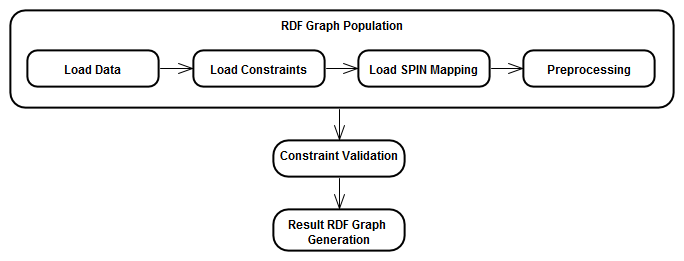
\includegraphics[width=1.00\textwidth]{constraint-validation-process.png}
	%\caption{Constraint Validation Process}
	%\label{fig:constraint-validation-process}
%\end{figure}

\begin{figure}[b]
\centerline{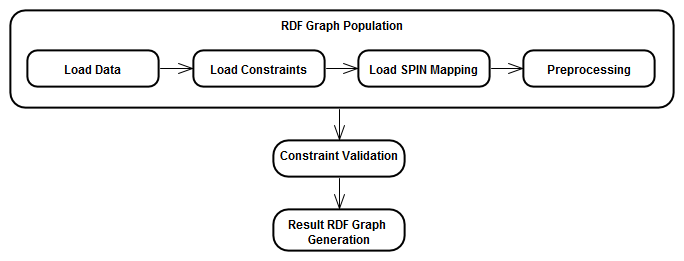
\psfig{file=constraint-validation-process.png,width=11cm}}
\vspace*{8pt}
\caption{Constraint Validation Process}
\label{fig:constraint-validation-process}
\end{figure}

First, an RDF graph has to be populated as follows:
\begin{enumerate}
\item The \emph{data} is loaded that is to be validated,
\item the \emph{constraints} in the DSCL are loaded,
\item the \emph{SPIN mapping} is loaded that contains the SPARQL representation of the DSCL, and 
\item the \emph{pre-processing} is performed, which can be provided in form of SPARQL CONSTRUCT queries.
\end{enumerate}

%When the input RDF graph is ready, the SPIN engine checks for each resource if it satisfies all constraints defined in the DSCL and generates a result RDF graph containing information about all constraint violations. With this framework, we have all we need to implement our own DSCL. 

When the input RDF graph is ready, the SPIN engine checks for each resource if it satisfies all constraints defined in the DSCL and associated with the classes assigned to the resource, and generates a result RDF graph containing information about all constraint violations.
With this framework, we have all we need to implement our own DSCL.

%With this implementation, there is one obvious limitation of our approach: the DSCL needs an RDF serialization. For OWL, DSP, ShEx, and ReSh, this is the case, but in the future, we would like to support non-RDF based languages as well. 
With this implementation, there are two obvious limitations of our approach: (1) constraints must be representable in RDF and (2) constraint languages must be expressible in SPARQL, i.e., the actual checking of constraints of each type the language supports must be expressible in form of a SPARQL query. For OWL 2, DSP, ShEx, ReSh, and SHACL, this is the case, but in the future, non-RDF based languages are expected to be supported as well. 

\subsection{Connect SPIN to your data}

A SPIN mapping consists of multiple \emph{SPIN construct templates} - each of them containing a SPARQL query executable to validate RDF data against constraints of a particular type. These templates are linked to the generic class \emph{ToValidate} whose instances are validated on constraints of a certain type expressed in the DSCL for which the mapping is defined:

\begin{ex}[commandchars=\\\{\}]
\textit{:ToValidate}
    spin:constraint 
        [ a dsp2spin:StatementTemplates_MinimumOccurrenceConstraint ] .
\end{ex}

As the mapping is designed to be independent of any concrete data, the class \emph{ToValidate} is purely generic. Instead of using such a generic class, it is also possible to link a template, responsible to check constraints of a given type, to the classes \emph{owl:Thing} or \emph{rdfs:Resource} to achieve that all instances of the input RDF graph are validated on constraints of that type. 

Neither of these classes has to be assigned manually and explicitly to instances within the data to be validated. They are either implicitly inferred by means of reasoning or explicitly assigned during the \emph{pre-processing} step, both in an automatic way. A reasonable approach would be to specify \emph{ToValidate} as super-class of all classes whose instances should actually be validated against constraints (in the case of DSP: classes that are linked via \ms{dsp:resourceClass} to a description template); this can be accomplished by a suitable SPARQL CONSTRUCT query that is executed before the validation starts. After \emph{pre-processing}, the data might look like in the following code snippet -- with the added assignment to the generic class in italics. 
%\emph{Description-Logic-Handbook} denotes a book with the subject \qs Computer Science\qe:

\begin{ex}[commandchars=\\\{\}]
:Description-Logic-Handbook
    a :Computer-Science-Book , \textit{:ToValidate} ;
    :subject "Computer Science" .
\end{ex}

\subsection{Mapping from a DSCL to SPIN}

The mapping from a DSCL to SPIN is performed by creating SPIN construct templates - one for each constraint type that is supported by the DSCL, so for the constraint type \emph{minimum unqualified cardinality restrictions (R-81)} expressible in DSP:
%a minimum occurrence that is required:

\begin{ex}[commandchars=\\\{\}]
dsp2spin:StatementTemplates_MinimumOccurrenceConstraint
    a \textit{spin:ConstructTemplate} ; 
    spin:body [
        a sp:Construct ;
        sp:templates (...) ;
        sp:where (...) ] .	
\end{ex}

\subsubsection{Representing validation results as constraint violations in RDF}

This is the general structure of a SPIN construct template representing a SPARQL CONSTRUCT query in RDF. We use SPARQL CONSTRUCT queries to generate descriptions for each detected constraint violation: 

\begin{ex}[commandchars=\\\{\}]
CONSTRUCT \{
    _:constraintViolation 
        a \textit{spin:ConstraintViolation} ;
        spin:violationRoot ?subject ;
        rdfs:label ?violationMessage ;
        spin:violationSource ?violationSource ;
        :severityLevel ?severityLevel ;
        spin:violationPath ?violationPath ;
        spin:fix ?violationFix \}
\end{ex}
%\pagebreak
In SPIN, the CONSTRUCT part of a SPARQL CONSTRUCT query is represented in RDF as follows:

\begin{ex}[commandchars=\\\{\}]
a \textit{sp:Construct} ;
sp:templates ( 
    [   sp:subject _:constraintViolation ; 
        sp:predicate rdf:type ; 
        sp:object spin:ConstraintViolation ]
    [   sp:subject _:constraintViolation ; 
        sp:predicate rdfs:label ; 
        sp:object [ sp:varName "violationMessage" ] ] ... ) ;
\end{ex}

Representing constraint violations and therefore validation results in RDF enables to process them further by means of Semantic Web technologies. SPIN construct templates generate constraint violation triples indicating the subject, the properties, and the constraints causing the violations and the reason why violations have been raised.

A SPIN construct template creates constraint violation triples if all triple patterns within the SPARQL WHERE clause of the SPARQL CONSTRUCT query match. If we specify the existential quantification that a book must have at least one author and if the book \emph{The-Hound-Of-The-Baskervilles} has no \emph{author} relationship, all the triple patterns within the SPARQL WHERE clause match and the SPIN construct template for checking constraints of the type \emph{existential quantifications (R-86)} generates a violation triple.

Constraint violations (\emph{spin:constraintViolation}) should provide useful messages (\emph{rdfs:label}) explaining the reasons why the data did not satisfy the constraint in order to assist data debugging and repair. In addition, constraint violation triples contain references to the subjects (\emph{spin:violationRoot}), the properties (\emph{spin:violationPath}), and the constraints (\emph{spin:violationSource}) causing the violations. In the example, the subject \emph{The-Hound-Of-The-Baskervilles}, the property \emph{author}, and the \emph{existential quantification} caused the violation. 

Constraint violation triples may be linked to useful messages explaining how to overcome raised violations. To fix constraint violations (\emph{spin:fix}), we may give some guidance how to become valid data either by adding, modifying, or deleting triples. To indicate how severe the violation of a constraint is, we introduce a new property to classify constraints according to different levels of severity (\emph{severityLevel}) like \emph{informational}, \emph{warning}, and \emph{error}. It is also important to find not validated triples, i.e., triples which have not been validated against any constraint, as it may be enforced that every triple of the input graph has to be validated.

%The SPARQL variable \emph{this} represents the current resource for which the constraint is checked.

\subsubsection{Representing constraint checks in RDF}

%As for the CONSTRUCT part of the SPARQL CONSTRUCT query, SPIN represents the WHERE clause, i.e., the actual check if constraints of a given type hold for the data, in RDF as well:
%
%\begin{ex}
%[   sp:subject [ sp:varName "subject" ] ; 
    %sp:predicate rdf:type ; 
    %sp:object [ sp:varName "resourceClass" ] ]
%\end{ex}

One of the main benefits of SPIN is that arbitrary SPARQL queries and thus constraint checks are representable as RDF triples. 
SPIN provides a vocabulary, the \emph{SPIN SPARQL Syntax}, to model SPARQL queries in RDF \cite{Knublauch-2011}. 
%The benefits of an RDF representation of constraint checks are:
%\begin{itemize}
%\item 
%Constraint checks can be consistently stored together with ontologies, constraints, and the data.
%\item
%Constraint checks can be easily shared on the Web of Data.
%\item
%Constraint validation can be executed automatically by a SPARQL execution engine.
%\item
%Constraint checks can directly be processed by a plethora of already existing RDF tools.
%\item
%Constraint checks are linkable to constraints and RDF data.
%\end{itemize}
An RDF representation of constraint checks enables that
(1) they can be consistently stored together with ontologies, constraints, and the data,
(2) they can easily be shared on the Web of Data,
(3) they can directly be processed by a plethora of already existing RDF tools,
(4) they are linkable to constraints and RDF data, and
(5) the validation of RDF data can automatically be executed by SPARQL execution engines.

As for the CONSTRUCT part of the SPARQL CONSTRUCT query, SPIN also represents the WHERE clause in RDF, i.e., the actual check if constraints of a given type hold for the data. The subsequent code snippet demonstrates how SPIN represents SPARQL 1.1 NOT EXISTS \cite{W3C-SPARQL1.1-Query-Language-2013} filter expressions in RDF ({\small\ms{FILTER NOT EXISTS \{ ?book author ?person \}}}) using the RDF Turtle syntax:

\begin{ex}[commandchars=\\\{\}]
[   a sp:Filter ;
    sp:expression [
        a sp:notExists ;
        sp:elements ( 
            [   sp:subject [ sp:varName "book" ] ;
                sp:predicate author ;
                sp:object [ sp:varName "person" ] ] ) ] ] )
\end{ex}

As the mapping of a DSCL to SPIN is defined for all constraint types supported by the DSCL and hence independently of concrete constraints, constraints of all these types are generally checked for each instance of the generic class \emph{ToValidate}. Therefore, the WHERE clause of a template always has to be restricted to classes for which concrete constraints are actually defined - in the case of DSP, the resource classes substituting the SPARQL variable \emph{?resourceClass}:

\begin{ex}
WHERE { ?subject rdf:type ?resourceClass . }
\end{ex}

\section{Evaluation}
\label{evaluation}

In this section, based on an automatic constraint checking of a large amount of RDF data sets, we formulate several findings to gain valuable insights and make recommendations to direct the further development of constraint languages.

Despite the large volume of the evaluated data sets in general, we have to keep in mind that in this study we only validate data against constraints for three vocabularies. We took all well-established and newly developed SBE vocabularies into account and defined constraints for the three vocabularies of them, which are most commonly used in the SBE sciences. For these three vocabularies, large data sets have already been published. For other SBE vocabularies, however, there is often not (yet) enough data openly available to draw general conclusions. Yet, these three vocabularies are representative, cover different aspects of SBE research data, and are also a mixture of widely adopted, accepted, and well-established vocabularies (QB and SKOS) on the one side and a vocabulary under development (DDI-RDF) on the other side. 

As the evaluation is based on only three vocabularies, we cannot make valid general statements for all vocabularies, but we can formulate several findings and make recommendations to direct the further development of constraint languages. As these findings cannot be proved yet, they still have to be verified or falsified by evaluating the quality of RDF data represented by further well-established and newly developed vocabularies - used within the SBE sciences and other domains.

\subsection{Experimental setup}

On the three vocabularies DDI-RDF, QB, and SKOS, we collected 115 constraints,\footnote{Implementations of all 115 constraints are online available at: \url{https://github.com/github-thomas-hartmann/phd-thesis/tree/master/chapter/chapter-9/constraints}} either from the vocabularies themselves or from several domain experts, and classified and implemented them for data validation. We ensured that these constraints are equally distributed over the sets and vocabularies we have. We then evaluated the data quality of 15,694 data sets (4.26 billion triples) of SBE research data, obtained from 33 SPARQL endpoints, by validating the data against these 115 constraints.
Table~\ref{tab:datasets} lists the number of validated data sets and the overall sizes in terms of validated triples for each of the vocabularies. 

\begin{table}[h]
		\scriptsize
    \begin{center}
		\caption{Number of Validated Data Sets and Triples for each Vocabulary}
		\label{tab:datasets}
    \begin{tabular}{llr}
%           & \multicolumn{6}{c}{\textbf{Vocabularies}}
%    \\  \cmidrule{2-7}
           \textbf{Vocabulary}
           & \textbf{Data Sets}
           & \textbf{Triples}
					 
    \\ \midrule
		%\emph{Triples} & 9,673,055 & 3,775,983,610 & 477,737,281 & 4,263,393,946 \\
		%\emph{Data Sets} & 1,526 & 9,990 & 4,178 & 15,694 \\
		%\hline
		\textbf{QB} & $9,990$   & $3,775,983,610$  \\
		\textbf{SKOS} & $4,178$  & $477,737,281$ \\
		\textbf{DDI-RDF} & $1,526$  & $9,673,055$  \\
    \bottomrule
    \end{tabular}
    %\\ \emph{C (constraints), CT (constraint types)}
    \end{center}
\end{table}

We validated, i.a., 
(1) QB data sets published by the \emph{Australian Bureau of Statistics},
the \emph{European Central Bank}, and the
\emph{Organisation for Economic Co-operation and Development},
(2) SKOS thesauri like the \emph{AGROVOC Multilingual agricultural thesaurus},
the \emph{STW Thesaurus for Economics}, and the
\emph{Thesaurus for the Social Sciences}, and
(3) DDI-RDF data sets provided by the \emph{Microdata Information System}, 
the \emph{Data Without Boundaries Discovery Portal}, the
\emph{Danish Data Archive}, and the
\emph{Swedish National Data Service}.
In a technical report, we describe the evaluation in further detail for each vocabulary, queried SPARQL endpoint, and constraint \cite{BoschZapilkoWackerowEckert2015-2}. Furthermore, we have published the evaluation results for each QB data set in form of one document per SPARQL endpoint.\footnote{Online available at: \url{https://github.com/github-thomas-hartmann/phd-thesis/tree/master/chapter/chapter-9/evaluation/data-sets/QB}}

%Since the validation of each of the 81 constraint types can be implemented using SPARQL, we use SPIN, a SPARQL-based way to formulate and check constraints, as basis to develop a
%validation environment to validate RDF data according to constraints expressed by arbitrary constraint languages.\footnote{Constraint language implementations online available at: \url{https://github.com/github-thomas-hartmann/phd-thesis/tree/master/rdf-validation/constraint-languages/implementations}}
%The \emph{RDF Validator}, online available at \url{http://purl.org/net/rdfval-demo}, can directly be used to validate arbitrary RDF data according to constraints extracted from the three vocabularies.\footnote{Vocabulary implementations online available at: \url{https://github.com/github-thomas-hartmann/phd-thesis/tree/master/rdf-validation/vocabularies/implementations}} Additionally, own constraints on any vocabulary can be defined using several constraint languages.
%
%The SPIN engine checks for each resource if it satisfies all constraints, which are associated with its assigned classes, and generates a result RDF graph containing information about all constraint violations.
%There is one SPIN construct template for each constraint type.
%A SPIN construct template contains a SPARQL CONSTRUCT query which generates constraint violation triples indicating the subject and the properties causing constraint violations and the reason why constraint violations have been raised.
%A SPIN construct template creates constraint violation triples if all triple patterns within the SPARQL WHERE clause match.

\subsection{Evaluation results and formulation of findings}

%DCAT: 11 constraints defined
%PHDD: 12
%XKOS: 10

%The majority (48 $\equiv$ 58.5\%) of the overall 81 $\mathcal{CT}$ constraint types are $\mathcal{CT}_{B}$ whose constraints can therefore be derived from vocabularies without any effort.
%Among $\mathcal{CT}_{B}$, two-thirds (34 $\equiv$ 70.8\%) are $\mathcal{C}_B ^{\mathcal{R}}$, i.e., constraint types for which reasoning may be performed prior to validation, and one third (14 $\equiv$ 29.2\%) are $\overline{\mathcal{C}_B ^{\mathcal{R}}}$, i.e., constraint types for which reasoning does not make any sense.
%A quarter (20 $\equiv$ 24.4\%) of all constraint types are $\mathcal{CT}_{S}$ and a sixth (14 $\equiv$ 17.1\%) are $\mathcal{CT}_{C}$.
%
%\begin{table}[H]
		%\scriptsize
    %\begin{center}
    %\begin{tabular}{@{}lcccc@{}}
%%           & \multicolumn{6}{c}{\textbf{Vocabularies}}
%%    \\  \cmidrule{2-7}
    %\\       \textbf{Criteria}
           %& \textbf{DDI-RDF}
           %& \textbf{QB}
					 %& \textbf{SKOS}
					 %& \textbf{Total}
    %\\ \midrule
		%%\emph{Triples} & 9,673,055 & 3,775,983,610 & 477,737,281 & 4,263,393,946 \\
		%%\emph{Data Sets} & 1,526 & 9,990 & 4,178 & 15,694 \\
		%%\hline
		%\emph{CT} & 52 & 20 & 15 & 53 \\
		%\hline
		%$\mathcal{CT}_{C}$ & 9 (17.3\%) & 2 (10\%) & 2 (13.3\%) & 9 (17\%) \\
		%$\mathcal{CT}_{S}$ & 16 (30.8\%) & 3 (15\%) & 4 (26,7\%) & 16 (30.2\%) \\
		%$\mathcal{CT}_{B}$ & 27 (\textbf{51.9\%}) & 15 (\textbf{75\%}) & 9 (\textbf{60\%}) & 28 (\textbf{52.8\%}) \\
		%\hline
		%$\mathcal{C}_B ^{\mathcal{R}}$ & 18 (34.6\%) & 9 (45\%) & 4 (26.7\%) & 19 (35.9\%) \\
		%$\overline{\mathcal{C}_B ^{\mathcal{R}}}$ & 9 (17.3\%) & 6 (30\%) & 5 (33.3\%) & 9 (17\%) \\
    %\bottomrule
    %\end{tabular}
    %%\\ \emph{C (constraints), CT (constraint types)}
    %\caption{Evaluation - Constraint Types}
		%\label{tab:evaluation-constraint-types}
    %\end{center}
%\end{table}

%Table \ref{tab:evaluation-constraint-types} displays the evaluation of the metadata quality on real world data sets regarding constraint types.
Tables \ref{tab:evaluation-constraint-violations-1} and \ref{tab:evaluation-constraint-violations-2} show the results of the evaluation, more specifically the numbers of constraints and constraint violations, which are caused by these constraints, in percent; whereas the numbers in the first line indicate the absolute amount of constraints and violations. The constraints and their raised violations are grouped by vocabulary, which type of language the types of the constraints are formulated with, and their severity level.

The numbers of validated triples and data sets differ between the vocabularies
as we validated 3.8 billion QB, 480 million SKOS, and 10 million DDI-RDF triples.
To be able to formulate findings which apply for all vocabularies, 
we only use normalized relative values representing the percentage of constraints and violations belonging to the respective sets. 

There is a strong overlap between \emph{RDFS/OWL} and \emph{Constraint Language Based} constraint types as in many cases constraint types are expressible by RDFS/OWL and classical constraint languages. This is the reason why the percentage values of constraints and violations grouped by the classification of constraint types according to the expressivity of constraint language types do not accumulate to 100\%. 

%\ke{da kam noch mal der limitations disclaimer, ich denke, einmal reicht... habs auskommentiert}
%As the evaluation is based on three vocabularies, 
%we cannot make valid general statements for all vocabularies,
%but we can formulate several findings to direct the further development of constraint languages.
%As these findings cannot be proved yet, 
%they still have to be verified or falsified
%by evaluating the quality of data represented by further well-established and newly developed vocabularies.

%by building the arithmetic mean over the individual vocabularies' percentage values. 
%\tb{More than 80\% of the overall approx. 55 million constraint violations are caused by QB constraints.}

%\begin{table}[H]
		%\scriptsize
    %\begin{center}
		%\caption{Constraints and Constraint Violations}
		%\label{tab:evaluation-constraint-violations}
    %\begin{tabular}{@{}lcccccccc@{}}
    %%       & \multicolumn{2}{c}{\textbf{Vocabularies}}
    %%\\  \cmidrule{2-3}
		%\hline
    %\multirow{2}{*}{} &
      %\multicolumn{2}{c}{\textbf{DDI-RDF}} &
      %\multicolumn{2}{c}{\textbf{QB}} &
      %\multicolumn{2}{c}{\textbf{SKOS}} &
      %\multicolumn{2}{c}{\textbf{\emph{Total}}} \\
    %\textbf{} & C & CV & C & CV & C & CV & C & CV \\
    %\hline
    %%\\ \midrule
		 %& 143 & 3,575,002 & 35 & 45,635,861 & 35 & 5,540,988 & 213 & 54,751,851 \\
		%\hline
		%\textbf{\emph{complex}} & 25.9\% & 18.3\% & 37.1\% & \textbf{100.0\%} & \textbf{37.1\%} & 21.4\% & 33.4\% & \textbf{46.6\%} \\
		%\textbf{\emph{simple}} & 19.6\% & 15.7\% & 8.6\% & 0.0\% & \textbf{34.3\%} & \textbf{78.6\%} & 20.8\% & 31.4\% \\
		%\textbf{\emph{vocabulary}} & \textbf{54.6\%} & \textbf{66.1\%} & \textbf{54.3\%} & 0.0\% & \textbf{28.6\%} & 0.0\% & \textbf{45.8\%} & 22.0\% \\
		%%\hline
		%%\emph{CV (}$\mathcal{C}_B ^{\mathcal{R}}$\emph{)} & 2,333,365 (65.3\%) & 1,777 (0\%) & 0 (0\%) & 2,335,142 (4.3\%) \\
		%%\emph{CV (}$\overline{\mathcal{C}_B ^{\mathcal{R}}}$\emph{)} & 28,000 (0.8\%) & 0 (0\%) & 0 (0\%) & 28,000 (0.1\%) \\
		%\hline
		%\textbf{\emph{info}} & \textbf{52.5\%} & \textbf{52.6\%} & 11.4\% & 0.0\% & \textbf{60.0\%} & 41.2\% & \textbf{41.3\%} & 31.3\% \\
		%\textbf{\emph{warning}} & 7.0\% & 29.4\% & 8.6\% & \textbf{99.8\%} & 14.3\% & \textbf{58.8\%} & 10.0\% & \textbf{62.7\%} \\
		%\textbf{\emph{error}} & 40.6\% & 18.0\% & \textbf{80.0\%} & 0.3\% & 25.7\% & 0.0\% & \textbf{48.8\%} & 6.1\%\\
    %\bottomrule
    %\end{tabular}
    %\\ \emph{C (constraints), CV (constraint violations)}
    %\end{center}
%\end{table}

%\begin{table}[H]
		%\scriptsize
    %\begin{center}
		%\caption{OLD}
		%\label{tab:evaluation-constraint-violations-1}
    %\begin{tabular}{@{}lcccc@{}}
    %%       & \multicolumn{2}{c}{\textbf{Vocabularies}}
    %%\\  \cmidrule{2-3}
		%\hline
    %\multirow{2}{*}{} &
      %\multicolumn{2}{c}{\textbf{DDI-RDF}} &
      %\multicolumn{2}{c}{\textbf{QB}} \\
    %\textbf{} & C & CV & C & CV \\
    %\hline
    %%\\ \midrule
		 %& 143 & 3,575,002 & 35 & 45,635,861 \\
		%\hline
		%\textbf{\emph{complex}} & 25.9\% & 18.3\% & 37.1\% & \textbf{100.0\%} \\
		%\textbf{\emph{simple}} & 19.6\% & 15.7\% & 8.6\% & 0.0\% \\
		%\textbf{\emph{vocabulary}} & \textbf{54.6\%} & \textbf{66.1\%} & \textbf{54.3\%} & 0.0\% \\
		%\hline
		%\textbf{\emph{info}} & \textbf{52.5\%} & \textbf{52.6\%} & 11.4\% & 0.0\% \\
		%\textbf{\emph{warning}} & 7.0\% & 29.4\% & 8.6\% & \textbf{99.8\%} \\
		%\textbf{\emph{error}} & 40.6\% & 18.0\% & \textbf{80.0\%} & 0.3\% \\
    %\bottomrule
    %\end{tabular}
    %\\ \emph{C (constraints), CV (constraint violations)}
    %\end{center}
%\end{table}
%
%\begin{table}[H]
		%\scriptsize
    %\begin{center}
		%\caption{OLD}
		%\label{tab:evaluation-constraint-violations-2}
    %\begin{tabular}{@{}lcccc@{}}
    %%       & \multicolumn{2}{c}{\textbf{Vocabularies}}
    %%\\  \cmidrule{2-3}
		%\hline
    %\multirow{2}{*}{} &
      %\multicolumn{2}{c}{\textbf{SKOS}} &
      %\multicolumn{2}{c}{\textbf{\emph{Total}}} \\
    %\textbf{} & C & CV & C & CV \\
    %\hline
    %%\\ \midrule
		 %& 35 & 5,540,988 & 213 & 54,751,851 \\
		%\hline
		%\textbf{\emph{complex}} & \textbf{37.1\%} & 21.4\% & 33.4\% & \textbf{46.6\%} \\
		%\textbf{\emph{simple}} & \textbf{34.3\%} & \textbf{78.6\%} & 20.8\% & 31.4\% \\
		%\textbf{\emph{vocabulary}} & \textbf{28.6\%} & 0.0\% & \textbf{45.8\%} & 22.0\% \\
		%\hline
		%\textbf{\emph{info}} & \textbf{60.0\%} & 41.2\% & \textbf{41.3\%} & 31.3\% \\
		%\textbf{\emph{warning}} & 14.3\% & \textbf{58.8\%} & 10.0\% & \textbf{62.7\%} \\
		%\textbf{\emph{error}} & 25.7\% & 0.0\% & \textbf{48.8\%} & 6.1\%\\
    %\bottomrule
    %\end{tabular}
    %\\ \emph{C (constraints), CV (constraint violations)}
    %\end{center}
%\end{table}

%\begin{table}[H]
		%\scriptsize
    %\begin{center}
		%\caption{Constraints and Constraint Violations (1)}
		%\label{tab:evaluation-constraint-violations-1}
    %\begin{tabular}{@{}lcccc@{}}
    %%       & \multicolumn{2}{c}{\textbf{Vocabularies}}
    %%\\  \cmidrule{2-3}
		%\hline
    %\multirow{2}{*}{} &
      %\multicolumn{2}{c}{\textbf{DDI-RDF}} &
      %\multicolumn{2}{c}{\textbf{QB}} \\
    %\textbf{} & C & CV & C & CV \\
    %\hline
    %%\\ \midrule
		 %& 143 & 3,575,002 & 35 & 45,635,861 \\
		%\hline
		%\textbf{\emph{SPARQL}} & 44.8\% & 34.7\% & \textbf{54.3\%} & \textbf{100.0\%} \\
		%\textbf{\emph{CL}} & 42.0\% & \textbf{65.3\%} & 28.6\% & 0.0\% \\
		%\textbf{\emph{RDFS/OWL}} & \textbf{51.8\%} & \textbf{65.3\%} & 42.9\% & 0.0\% \\
		%\hline
		%\textbf{\emph{info}} & \textbf{52.5\%} & \textbf{52.6\%} & 11.4\% & 0.0\% \\
		%\textbf{\emph{warning}} & 7.0\% & 29.4\% & 8.6\% & \textbf{99.8\%} \\
		%\textbf{\emph{error}} & 40.6\% & 18.0\% & \textbf{80.0\%} & 0.3\% \\
    %\bottomrule
    %\end{tabular}
    %\\ \emph{C (constraints), CV (constraint violations)}
    %\end{center}
%\end{table}
%
%\begin{table}[H]
		%\scriptsize
    %\begin{center}
		%\caption{Constraints and Constraint Violations (2)}
		%\label{tab:evaluation-constraint-violations-2}
    %\begin{tabular}{@{}lcccc@{}}
    %%       & \multicolumn{2}{c}{\textbf{Vocabularies}}
    %%\\  \cmidrule{2-3}
		%\hline
    %\multirow{2}{*}{} &
      %\multicolumn{2}{c}{\textbf{SKOS}} &
      %\multicolumn{2}{c}{\textbf{\emph{Total}}} \\
    %\textbf{} & C & CV & C & CV \\
    %\hline
    %%\\ \midrule
		 %& 35 & 5,540,988 & 213 & 54,751,851 \\
		%\hline
		%\textbf{\emph{SPARQL}} & \textbf{80.0\%} & \textbf{100.0\%} & \textbf{59.7\%} & \textbf{78.2\%} \\
		%\textbf{\emph{CL}} & 0.0\% & 0.0\% & 23.5\% & 21.8\% \\
		%\textbf{\emph{RDFS/OWL}} & 20.0\% & 0.0\% & 38.2\% & 21.8\% \\
		%\hline
		%\textbf{\emph{info}} & \textbf{60.0\%} & 41.2\% & \textbf{41.3\%} & 31.3\% \\
		%\textbf{\emph{warning}} & 14.3\% & \textbf{58.8\%} & 10.0\% & \textbf{62.7\%} \\
		%\textbf{\emph{error}} & 25.7\% & 0.0\% & \textbf{48.8\%} & 6.1\%\\
    %\bottomrule
    %\end{tabular}
    %\\ \emph{C (constraints), CV (constraint violations)}
    %\end{center}
%\end{table}

\begin{table}[h]
		\scriptsize
    \begin{center}
		\caption{Evaluation Results (1)}
		\label{tab:evaluation-constraint-violations-1}
    \begin{tabular}{@{}lcc|cc@{}}
    %       & \multicolumn{2}{c}{\textbf{Vocabularies}}
    %\\  \cmidrule{2-3}
		%\hline
    \multirow{2}{*}{} &
      \multicolumn{2}{c}{\textbf{DDI-RDF}} &
      \multicolumn{2}{c}{\textbf{QB}} \\
    \textbf{} & C & CV & C & CV \\
    \hline
    %\\ \midrule
		 & 78 & 3,575,002 & 20 & 45,635,861 \\
		\hline
		\textbf{\emph{SPARQL}} & 29.5 & 34.7 & \textbf{60.0} & \textbf{100.0} \\
		\textbf{\emph{CL}} & \textbf{64.1} & \textbf{65.3} & 40.0 & 0.0 \\
		\textbf{\emph{RDFS/OWL}} & \textbf{66.7} & \textbf{65.3} & 40.0 & 0.0 \\
		\hline
		\textbf{\emph{info}} & \textbf{56.4} & \textbf{52.6} & 0.0 & 0.0 \\
		\textbf{\emph{warning}} & 11.5 & 29.4 & 15.0 & \textbf{99.8} \\
		\textbf{\emph{error}} & 32.1 & 18.0 & \textbf{85.0} & 0.3 \\
    \bottomrule
    \end{tabular}
    \\ \emph{C (constraints), CV (constraint violations)}
    \end{center}
\end{table}

\begin{table}[h]
		\scriptsize
    \begin{center}
		\caption{Evaluation Results (2)}
		\label{tab:evaluation-constraint-violations-2}
    \begin{tabular}{@{}lcc|cc@{}}
    %       & \multicolumn{2}{c}{\textbf{Vocabularies}}
    %\\  \cmidrule{2-3}
		%\hline
    \multirow{2}{*}{} &
      \multicolumn{2}{c}{\textbf{SKOS}} &
      \multicolumn{2}{c}{\textbf{\emph{Total}}} \\
    \textbf{} & C & CV & C & CV \\
    \hline
    %\\ \midrule
		 & 17 & 5,540,988 & 115 & 54,751,851 \\
		\hline
		\textbf{\emph{SPARQL}} & \textbf{100.0} & \textbf{100.0} & \textbf{63.2} & \textbf{78.2} \\
		\textbf{\emph{CL}} & 0.0 & 0.0 & 34.7 & 21.8 \\
		\textbf{\emph{RDFS/OWL}} & 0.0 & 0.0 & 35.6 & 21.8 \\
		\hline
		\textbf{\emph{info}} & \textbf{70.6} & 41.2 & \textbf{42.3} & 31.3 \\
		\textbf{\emph{warning}} & 29.4 & \textbf{58.8} & 18.7 & \textbf{62.7} \\
		\textbf{\emph{error}} & 0.0 & 0.0 & \textbf{39.0} & 6.1\\
    \bottomrule
    \end{tabular}
    \\ \emph{C (constraints), CV (constraint violations)}
    \end{center}
\end{table}

%More than the half of them are $\mathcal{CT}_{B}$, nearly a third $\mathcal{CT}_{S}$, and only a sixth $\mathcal{CT}_{C}$ constraint types.
%For DDI-RDF, QB, and SKOS, more than 50\% of the instantiated constraint types are $\mathcal{CT}_{B}$ constraint types 
%(for QB even three quarters).
%\emph{Existential quantifications} (\emph{R-86}, 32.4\%, DDI-RDF), \emph{data model consistency} (31.4\%, QB), and \emph{structure} (28.6\%, SKOS) are the constraint types the most constraints are instantiated from.
%\tb{1. Fakten (diese Fakten bewirken eine Erhöhung der Datenqualität) 2. Hypothese (unsere Interpretation der Ergebnisse, unsere Behauptung)}

Almost 2/3 of all constraints, nearly 1/3 of the DDI-RDF, 60\% of the QB, and all SKOS constraints are \emph{SPARQL Based}. For well-established vocabularies, the most formulated constraints are \emph{SPARQL Based} (80\%). For newly developed vocabularies, however, the most expressed constraints are \emph{RDFS/OWL Based} (2/3). 
%
Nearly 80\% of all violations are caused by \emph{SPARQL}, 1/5 by \emph{Constraint Language}, and 1/5 by \emph{RDFS/OWL Based} constraints.
%Hence, a significant amount of 46 \% of the constraints are directly extractable from formal specifications of well-established and newly defined vocabularies. 
%\begin{hyp}
%As a significant amount of 46 \% of the constraints are vocabulary constraints which can be expressed by modeling languages like RDF, RDFS, and OWL 2,
%the further development of constraint languages should concentrate on expressing simple and especially complex constraints which up to now in most cases can only be expressed by plain SPARQL.   
%As a significant amount of 54\% of the constraints are either simple or complex constraints,
%the further development of constraint languages should concentrate on expressing simple and especially complex constraints which up to now in most cases can only be expressed by plain SPARQL.  
%\end{hyp}
\par\bigskip
{\centering\textbf{Finding 1}}
\emph{The facts that 80\% of all violations are raised by SPARQL Based constraints and that 2/3 of all constraints are SPARQL Based, increases the importance to formulate constraints, which up to now can only be expressed in SPARQL, using high-level constraint languages. Data quality can be significantly improved when suitable constraint languages are developed which enable to define SPARQL Based constraints in an easy, concise, and intuitive way. Thereby, the more elaborate a vocabulary is, the more sophisticated and complex constraints are specified using SPARQL.}
\par\bigskip

These constraints are of such complexity that up to now in most cases they can only be expressed by plain SPARQL. It should be an incentive for language designers to devise languages which are more intuitive than SPARQL in a way that also domain experts, which are not familiar with SPARQL, can formulate respective constraints.

%Nearly 1/3 of all constraints are either \emph{RDFS/OWL} or \emph{Constraint Language Based}.

%The fact that only 1/5 of all violations result from \emph{RDFS/OWL Based} constraints, even though 1/3 of all constraints are \emph{RDFS/OWL Based}, indicates good data quality for all vocabularies with regard to their formal specifications.

\par\bigskip
{\centering\textbf{Finding 2}}
\emph{The fact that only 1/5 of all violations result from RDFS/OWL Based constraints, even though more than 1/3 of all constraints are RDFS/OWL Based, indicates good data quality for all vocabularies with regard to their formal specifications.}
\par\bigskip

{\centering\textbf{Finding 3}}
\emph{As more than 1/3 of all constraints are RDFS/OWL Based, the first step to make progress in the further development of constraint languages is to cover the constraint types which can already be formulated using RDFS and OWL.}
\par\bigskip

%\tb{je nach hypothese spezifische aufgaben um die hypothese zu beweisen}
While 2/3 of the DDI-RDF violations result from \emph{RDFS/OWL Based} constraints,
QB and SKOS violations are only raised by \emph{SPARQL Based} constraints.

\par\bigskip
{\centering\textbf{Finding 4}}
\emph{For well-established vocabularies, RDFS/OWL Based constraints are almost completely satisfied which generally indicates very impressive data quality, at least in the SBE domain and for the basic requirements. For newly developed vocabularies, however, data quality is poor as RDFS/OWL Based constraints are not fulfilled.}
\par\bigskip

For DDI-RDF, data providers still have to understand the vocabulary and of course data cannot have high quality if the specification is not yet stable.
It is likely that a newly developed vocabulary is still subject of constant change
and that early adopters did not properly understand its formal specification.
Thus, published data may not be consistent with the current draft of its conforming vocabulary.

When vocabularies under development turn into well-established ones,
data providers are experienced in publishing their data in conformance with these vocabularies
and formal specifications are more elaborated. 
As a consequence, \emph{RDFS/OWL Based} constraints are satisfied to a greater extend which leads to better data quality.  

The reason why we only defined \emph{SPARQL Based} constraints on SKOS for assessing the quality of thesauri is that literature and practice especially concentrate on evaluating graph-based structures of thesauri by applying graph- and network-analysis techniques which are of such complexity that they can only be implemented in SPARQL.

%Therefore, existing constraint languages have to be extended or new constraint languages have to be developed.

%\begin{table}[H]
		%\scriptsize
    %\begin{center}
		%\caption{Constraints and Constraint Violations (1)}
		%\label{tab:evaluation-constraint-violations-1}
    %\begin{tabular}{@{}lcccc@{}}
    %%       & \multicolumn{2}{c}{\textbf{Vocabularies}}
    %%\\  \cmidrule{2-3}
		%\hline
    %\multirow{2}{*}{} &
      %\multicolumn{2}{c}{\textbf{DDI-RDF}} &
      %\multicolumn{2}{c}{\textbf{QB}} \\
    %\textbf{} & C & CV & C & CV \\
    %\hline
    %%\\ \midrule
		 %& 143 & 3,575,002 & 35 & 45,635,861 \\
		%\hline
		%\textbf{\emph{SPARQL}} & 44.8\% & 34.7\% & \textbf{54.3\%} & \textbf{100.0\%} \\
		%\textbf{\emph{CL}} & 42.0\% & \textbf{65.3\%} & 28.6\% & 0.0\% \\
		%\textbf{\emph{RDFS/OWL}} & \textbf{51.8\%} & \textbf{65.3\%} & 42.9\% & 0.0\% \\
		%\hline
		%\textbf{\emph{info}} & \textbf{52.5\%} & \textbf{52.6\%} & 11.4\% & 0.0\% \\
		%\textbf{\emph{warning}} & 7.0\% & 29.4\% & 8.6\% & \textbf{99.8\%} \\
		%\textbf{\emph{error}} & 40.6\% & 18.0\% & \textbf{80.0\%} & 0.3\% \\
    %\bottomrule
    %\end{tabular}
    %\\ \emph{C (constraints), CV (constraint violations)}
    %\end{center}
%\end{table}
%
%\begin{table}[H]
		%\scriptsize
    %\begin{center}
		%\caption{Constraints and Constraint Violations (2)}
		%\label{tab:evaluation-constraint-violations-2}
    %\begin{tabular}{@{}lcccc@{}}
    %%       & \multicolumn{2}{c}{\textbf{Vocabularies}}
    %%\\  \cmidrule{2-3}
		%\hline
    %\multirow{2}{*}{} &
      %\multicolumn{2}{c}{\textbf{SKOS}} &
      %\multicolumn{2}{c}{\textbf{\emph{Total}}} \\
    %\textbf{} & C & CV & C & CV \\
    %\hline
    %%\\ \midrule
		 %& 35 & 5,540,988 & 213 & 54,751,851 \\
		%\hline
		%\textbf{\emph{SPARQL}} & \textbf{80.0\%} & \textbf{100.0\%} & \textbf{59.7\%} & \textbf{78.2\%} \\
		%\textbf{\emph{CL}} & 0.0\% & 0.0\% & 23.5\% & 21.8\% \\
		%\textbf{\emph{RDFS/OWL}} & 20.0\% & 0.0\% & 38.2\% & 21.8\% \\
		%\hline
		%\textbf{\emph{info}} & \textbf{60.0\%} & 41.2\% & \textbf{41.3\%} & 31.3\% \\
		%\textbf{\emph{warning}} & 14.3\% & \textbf{58.8\%} & 10.0\% & \textbf{62.7\%} \\
		%\textbf{\emph{error}} & 25.7\% & 0.0\% & \textbf{48.8\%} & 6.1\%\\
    %\bottomrule
    %\end{tabular}
    %\\ \emph{C (constraints), CV (constraint violations)}
    %\end{center}
%\end{table}

Almost 40\% of all constraints are \emph{error}, more than 40\% are \emph{informational}, and nearly 20\% are \emph{warning} constraints.
\emph{Informational} constraints caused approximately 1/3 and
\emph{warning} constraints narrowly 2/3 of all violations.
%As the percentage of severe violations is very low for all vocabularies (6.1\%),
%data quality is high with regard to the severity level of constraints.

\par\bigskip
{\centering\textbf{Finding 5}}
\emph{Although 40\% of all constraints are error constraints, the percentage of severe violations is very low, compared to about 2/3 of warning and 1/3 of informational violations. This implies that data quality is high with regard to the severity level of constraints and that proper constraint languages can significantly improve data quality beyond fundamental requirements.}
\par\bigskip

We did not detect violations of \emph{error} constraints for well-established vocabularies, even though 85\% of the QB constraints are \emph{error} constraints. 
%85\% of the QB constraints are \emph{error} constraints.
More than 50\% of the DDI-RDF constraints and more than 70\% of the SKOS constraints are \emph{informational} constraints.
1/6 of the DDI-RDF violations are caused by \emph{error} constraints and
almost all QB and 59\% of the SKOS violations are caused by \emph{warning} constraints. 
%For well-established vocabularies, we detected no violations of \emph{error} constraints.  
%Constraints are serious when they violate the integrity of vocabularies.
%For well-established vocabularies, it is well documented and the experience is high how to guarantee this integrity
%which is not the case or newly-developed vocabularies.

\par\bigskip
{\centering\textbf{Finding 6}}
\emph{For well-established vocabularies, data quality is high as serious violations rarely appear (0.3\% for QB). For newly developed vocabularies, however, data quality is worse as serious violations occur partially (1/6 for DDI-RDF).}
\par\bigskip

Especially for vocabularies under development, constraint languages should be used to a larger extend in addition to RDFS/OWL in order to define appropriate constraints to detect and solve severe violations.
%\ke{aber das wird doch gemacht, halt mit RDFS und OWL, weswegen die etablierten ja besser sind.}
%to reduce severe violations by checking and solving them.

%For the vocabularies DDI-RDF, QB, and SKOS, we defined 213 constraints of 53 constraint types .

%\begin{table}[H]
		%\scriptsize
    %\begin{center}
    %\begin{tabular}{@{}lcccc@{}}
%%           & \multicolumn{6}{c}{\textbf{Vocabularies}}
%%    \\  \cmidrule{2-7}
    %\\       \textbf{Criteria}
           %& \textbf{DDI-RDF}
           %& \textbf{QB}
					 %& \textbf{SKOS}
					 %& \textbf{Total}
    %\\ \midrule
		%%\emph{Triples} & 9,673,055 & 3,775,983,610 & 477,737,281 & 4,263,393,946 \\
		%%\emph{Data Sets} & 1,526 & 9,990 & 4,178 & 15,694 \\
		%%\hline
		%\emph{C} & 143 (67.1\%) & 35 (16.4\%) & 35 (16.4\%) & 213 \\
		%\hline
		%\emph{C (}$\mathcal{CT}_{C}$\emph{)} & 37 (25.9\%) & 13 (37.1\%) & 13 (\textbf{37.1\%}) & 63 (29.6\%) \\
		%\emph{C (}$\mathcal{CT}_{S}$\emph{)} & 28 (19.6\%) & 3 (8.6\%) & 12 (\textbf{34.3\%}) & 43 (20.2\%) \\
		%\emph{C (}$\mathcal{CT}_{B}$\emph{)} & 78 (\textbf{54.6\%}) & 19 (\textbf{54.3\%}) & 10 (\textbf{28.6\%}) & 107 (\textbf{50.2\%}) \\
		%%\hline
		%%\emph{C (}$\mathcal{C}_B ^{\mathcal{R}}$\emph{)} & 67 (46.9\%) & 13 (37.1\%) & 4 (11.4\%) & 84 (39.4\%) \\
		%%\emph{C (}$\overline{\mathcal{C}_B ^{\mathcal{R}}}$\emph{)} & 11 (7.7\%) & 6 (17.1\%) & 6 (17.1\%) & 23 (10.8\%) \\
		%\hline
		%\emph{C ($\mathcal{SL}_{0}$)} & 75 (\textbf{52.5\%}) & 4 (11.4\%) & 21 (\textbf{60\%}) & 100 (\textbf{46.9\%}) \\
		%\emph{C ($\mathcal{SL}_{1}$)} & 10 (7\%) & 3 (8.6\%) & 5 (14.3\%) & 18 (8.5\%) \\
		%\emph{C ($\mathcal{SL}_{2}$)} & 58 (40.6\%) & 28 (\textbf{80\%}) & 9 (25.7\%) & 95 (\textbf{44.6\%}) \\
    %\bottomrule
    %\end{tabular}
    %%\\ \emph{C (constraints), CT (constraint types)}
    %\caption{Evaluation - Constraints}
		%\label{tab:evaluation-constraints}
    %\end{center}
%\end{table}





%\begin{table}[H]
		%\scriptsize
    %\begin{center}
    %\begin{tabular}{@{}lcccccccc@{}}
%%           & \multicolumn{6}{c}{\textbf{Vocabularies}}
%%    \\  \cmidrule{2-7}
    %\\       \textbf{}
           %& \textbf{DDI-RDF}
           %& \textbf{QB}
					 %& \textbf{SKOS}
					 %& \textbf{Total}
					 %& \textbf{DDI-RDF}
           %& \textbf{QB}
					 %& \textbf{SKOS}
					 %& \textbf{Total}
    %\\ \midrule
		 %& 3,575,002 & 45,635,861 & 5,540,988 & 54,751,851 & & & &  \\
		%\hline
		%\textbf{\emph{complex}} & 18.3\% & \textbf{100\%} & 21.4\% & \textbf{86.7\%} & & & & \\
		%\textbf{\emph{simple}} & 15.7\% & 0.0\% & \textbf{78.6\%} & 9\% & & & & \\
		%\textbf{\emph{vocabulary}} & \textbf{66.1\%} & 0.0\% & 0\% & 4.3\% & & & & \\
		%%\hline
		%%\emph{CV (}$\mathcal{C}_B ^{\mathcal{R}}$\emph{)} & 2,333,365 (65.3\%) & 1,777 (0\%) & 0 (0\%) & 2,335,142 (4.3\%) \\
		%%\emph{CV (}$\overline{\mathcal{C}_B ^{\mathcal{R}}}$\emph{)} & 28,000 (0.8\%) & 0 (0\%) & 0 (0\%) & 28,000 (0.1\%) \\
		%\hline
		%\textbf{\emph{info}} & \textbf{52.6\%} & 0.0\% & 41.2\% & 7.6\% & & & & \\
		%\textbf{\emph{warning}} & 29.4\% & \textbf{99,8\%} & \textbf{58.8\%} & \textbf{91\%} & & & & \\
		%\textbf{\emph{error}} & 18\% & 0.3\% & 0.0\% & 1.4\% & & & & \\
    %\bottomrule
    %\end{tabular}
    %%\\ \emph{CV (constraint violations)}
    %\caption{Constraint Violations}
		%\label{tab:evaluation-constraint-violations}
    %\end{center}
%\end{table}

%The constraints responsible for the largest amounts of constraint violations are \emph{DDI-RDF-C-LABELING-AND-DOCUMENTATION-06} and \emph{DDI-RDF-C-COMPARISON-VARIABLES-02} (both 547,916; DDI-RDF), \emph{DATA-CUBE-C-DATA-MODEL-CONSISTENCY-05} (45,514,102; QB), and \emph{SKOS-C-LANGUAGE-TAG-CARDINALITY-01} (2,508,903; SKOS).

%Table \ref{tab:evaluation-expressivity-severity} shows the relations between the severity level of the violations caused by all 115 constraints and the classification according to the expressivity of constraint languages of the constraint types of the violations in percent. 
80\% of the violations, which are raised by either \emph{RDFS/OWL} or \emph{Constraint Language Based} constraints, are caused by constraints with the severity level \emph{informational} (see Table \ref{tab:evaluation-expressivity-severity}) and almost all (94\%) of the violations, which are caused by \emph{SPARQL Based} constraints, are raised by \emph{warning} constraints. Approximately 1/2 of all constraints are \emph{informational} constraints regardless how their types are classified according to the expressivity of constraint language types.

%\begin{table}[H]
		%\scriptsize
    %\begin{center}
		%\caption{OLD}
		%\label{tab:evaluation-complexity-severity}
    %\begin{tabular}{@{}lcccc@{}}
%%           & \multicolumn{6}{c}{\textbf{Vocabularies}}
%%    \\  \cmidrule{2-7}
    %\\       \textbf{}
           %& \textbf{\emph{RDFS/OWL}}
           %& \textbf{\emph{Constraint Language}}
					 %& \textbf{\emph{SPARQL}}
    %\\ \midrule
		%%\emph{Triples} & 9,673,055 & 3,775,983,610 & 477,737,281 & 4,263,393,946 \\
		%%\emph{Data Sets} & 1,526 & 9,990 & 4,178 & 15,694 \\
		%%\hline
		%\textbf{\emph{info}} & 38.7 \% & \textbf{76.2 \%} & \textbf{42.3 \%} \\
		%\textbf{\emph{warning}} & 6.7 \% & 7.1 \% & 13.5 \% \\
		%\textbf{\emph{error}} & \textbf{54.6 \%} & 16.7 \% & \textbf{44.2 \%} \\
    %\bottomrule
    %\end{tabular}
    %%\\ \emph{C (constraints), CT (constraint types)}
    %\end{center}
%\end{table}

%\begin{table}[H]
		%\scriptsize
    %\begin{center}
		%\caption{Constraint Language Expressivity and Severity Level of Violations}
		%\label{tab:evaluation-violations-expressivity-severity}
    %\begin{tabular}{@{}lcccc@{}}
%%           & \multicolumn{6}{c}{\textbf{Vocabularies}}
%%    \\  \cmidrule{2-7}
    %\\       \textbf{}
           %& \textbf{\emph{RDFS/OWL}}
           %& \textbf{\emph{Constraint Language}}
					 %& \textbf{\emph{SPARQL}}
    %\\ \midrule
		%%\emph{Triples} & 9,673,055 & 3,775,983,610 & 477,737,281 & 4,263,393,946 \\
		%%\emph{Data Sets} & 1,526 & 9,990 & 4,178 & 15,694 \\
		%%\hline
		%\textbf{\emph{info}} & \textbf{79.64} & \textbf{79.60} & 4.39 \\
		%\textbf{\emph{warning}} & 20.28 & 20.27 & \textbf{94.17} \\
		%\textbf{\emph{error}} & 0.08 & 0.13 & 1.43 \\
    %\bottomrule
    %\end{tabular}
    %%\\ \emph{C (constraints), CT (constraint types)}
    %\end{center}
%\end{table}

%\begin{table}[H]
		%\scriptsize
    %\begin{center}
		%\caption{Constraint Language Expressivity and Severity Level of Constraints}
		%\label{tab:evaluation-constraints-expressivity-severity}
    %\begin{tabular}{@{}lcccc@{}}
%%           & \multicolumn{6}{c}{\textbf{Vocabularies}}
%%    \\  \cmidrule{2-7}
    %\\       \textbf{}
           %& \textbf{\emph{RDFS/OWL}}
           %& \textbf{\emph{Constraint Language}}
					 %& \textbf{\emph{SPARQL}}
    %\\ \midrule
		%%\emph{Triples} & 9,673,055 & 3,775,983,610 & 477,737,281 & 4,263,393,946 \\
		%%\emph{Data Sets} & 1,526 & 9,990 & 4,178 & 15,694 \\
		%%\hline
		%\textbf{\emph{info}} & \textbf{79.64} & \textbf{79.60} & 4.39 \\
		%\textbf{\emph{warning}} & 20.28 & 20.27 & \textbf{94.17} \\
		%\textbf{\emph{error}} & 0.08 & 0.13 & 1.43 \\
    %\bottomrule
    %\end{tabular}
    %%\\ \emph{C (constraints), CT (constraint types)}
    %\end{center}
%\end{table}

\begin{table}[h]
		\scriptsize
    \begin{center}
		\caption{Constraints and Violations by Language Type and Severity}
		\label{tab:evaluation-expressivity-severity}
    \begin{tabular}{@{}lcc|cc|cc@{}}
    %       & \multicolumn{2}{c}{\textbf{Vocabularies}}
    %\\  \cmidrule{2-3}
		%\hline
    \multirow{3}{*}{} &
      \multicolumn{2}{c}{\textbf{RDFS/OWL}} &
      \multicolumn{2}{c}{\textbf{\emph{CL}}} &
      \multicolumn{2}{c}{\textbf{\emph{SPARQL}}} \\
    \textbf{} & C & CV & C & CV & C & CV \\
    \hline
		\textbf{\emph{info}} & \textbf{52.5} & \textbf{79.64} & \textbf{55.2} & \textbf{79.60} & \textbf{45.1} & 4.39 \\
		\textbf{\emph{warning}} & 18.0 & 20.28 & 15.5 & 20.27 & 19.6 & \textbf{94.17} \\
		\textbf{\emph{error}} & 29.5 & 0.08 & 29.3 & 0.13 & 35.3 & 1.43 \\
    \bottomrule
    \end{tabular}
		\\ \emph{C (constraints), CV (constraint violations)}
    \end{center}
\end{table}

\par\bigskip
{\centering\textbf{Finding 7}}
\emph{Whatever language is used to formulate constraints, 1/2 of all constraints are informational, 1/3 are error, and 1/5 are warning constraints.}
\par\bigskip

The fact, that regardless of the language used to specify constraints, 1/2 of all constraints are \emph{informational} 
%indicates that the purpose of constraints for users is mostly just to point to desirable but not necessary data improvements in terms of syntax and semantics of vocabularies. 
indicates the importance that constraint languages support
constraints on multiple levels. Constraints are by far not only used to
prevent certain usages of a vocabulary, they are rather needed to
provide better guidance for improved interoperability.

\par\bigskip
{\centering\textbf{Finding 8}}
\emph{Regardless of the type of the used language, there are only a few violations raised by error constraints which stands for good data quality in general.
In contrast, constraints of low severity, expressible by RDFS/OWL or high-level constraint languages, are violated to a large extent (80\%), whereas more serious warning constraints, only expressible by SPARQL, are violated to an even larger extend (94\%).}
\par\bigskip

%The reason why there is a significant demand for languages supporting \emph{SPARQL Based} constraints is that 94\% of all violations, which are caused by \emph{SPARQL Based} constraints, are also raised by \emph{warning} constraints. This means that data quality may be improved in case these \emph{warning} constraints are adequately tackled which is more likely when these constraints are expressible not only by SPARQL but also by high-level constraint languages enabling to formulate constraints more intuitively and concisely. 

94\% of the violations caused by \emph{SPARQL Based} constraints are \emph{warnings}, which
means that data quality could be significantly improved when solving these quite serious violations. We claim that this is more likely when these \emph{SPARQL Based} constraints 
are not only expressible by plain SPARQL but also by high-level
constraint languages enabling to formulate such constraints in a more
intuitive and concise way.

\section{Conclusion and Future Work}

%In this paper, we showed in form of a complete real world running example how to represent metadata on unit-record data (DDI-RDF), metadata on aggregated data (QB), and data on both aggregation levels in a rectangular format (\emph{PHDD}) in RDF and how therefore used vocabularies are interrelated (\textbf{contribution 1}, section \ref{rdf-representation}).
%We explained why RDF validation is important in this context and how metadata on unit-record data, aggregated data, thesauri, and statistical classifications as well as data on both aggregation levels is validated against constraints to ensure high (meta)data quality\footnote{The first appendix of this paper describing each constraint in detail is available at: \url{http://arxiv.org/abs/1504.04479} \cite{BoschZapilkoWackerowEckert2015}} (\textbf{contribution 2}, section \ref{rdf-validation}). 
%We distinguish two validation types:
%(1) \emph{Content-Driven Validation} $\mathcal{C}_{C}$ contains the set of constraints ensuring that the data is consistent with the intended syntax, semantics, and integrity of data models (section \ref{SPARQL-based-constraint-types}).
%(2) \emph{Technology-Driven Validation} $\mathcal{C}_{T}$ includes the set of constraints which can be generated automatically out of data models, such as cardinality restrictions, universal and existential quantifications, domains, and ranges (section \ref{vocabulary-constraint-types}).
%We determined the default \emph{severity level} for each constraint to indicate how serious the violation of the constraint is
%and propose an extensible metric to measure the continuum of severity levels.

%We implemented a validation environment (available at \url{http://purl.org/net/rdfval-demo}) to validate RDF data according to constraints expressed my arbitrary constraint languages and to ensure correct syntax and semantics of diverse vocabularies such as DDI-RDF, QB, SKOS, and \emph{PHDD} (section \ref{implementation}).
%We exhaustively evaluated the metadata quality of large real world aggregated (QB), unit-record (DDI-RDF), and thesauri (SKOS) data sets (more than 4.2 billion triples and 15 thousand data sets) by means of 213  constraints of the majority of the constraint types\footnote{The second appendix of this paper describing the evaluation in detail is available at: \url{http://arxiv.org/abs/1504.04478} \cite{BoschZapilkoWackerowEckert2015-2}.} (section \ref{evaluation}).

We captured 115 constraints on three vocabularies commonly used within the social, behavioral, and economic (SBE) sciences (DDI-RDF, QB, and SKOS), either from the vocabularies themselves or from several domain experts, and classified them based on by which of the three types of constraint languages (\emph{RDFS/OWL Based}, \emph{Constraint Language Based}, and \emph{SPARQL Based}) their constraint types can be expressed. 

In addition, we let the domain experts classify each constraint according to the severity of its violation.
Although we provide default severity levels for each constraint, validation environments should enable users to adapt the severity levels of constraints according to their individual needs.
We simplify the classification system of log messages in software development and differentiate between the three severity levels \emph{informational}, \emph{warning}, and \emph{error}.

By validating against these constraints, we evaluated  the data quality of 15,694 data sets (4.26 billion triples) of SBE research data, obtained from 33 SPARQL endpoints. This way, we gain a better understanding about the role of certain constraint types for assessing the quality of RDF data and therefore the usability of identified constraint types for determining RDF data quality.

Based on the evaluation results, we formulated several findings to direct the further development of constraint languages. The general applicability of these findings, however, is still to be confirmed beyond the examined vocabularies and for other domains.
The main findings are: 

\begin{enumerate}
\item
\emph{Data quality can be significantly improved when suitable constraint languages are developed enabling to define 
constraints - which up to now can only be expressed by plain SPARQL - in an easy, concise, and intuitive way. Thereby, the more elaborate a vocabulary is, the more sophisticated and complex constraints are necessary, which in most cases can only be specified in SPARQL.}
\item
\emph{As only 1/5 of all violations result from constraints which are expressible in RDFS or OWL, even though 1/3 of all constraints are representable in RDFS/OWL, data quality is high for all vocabularies with regard to their formal specifications.}  
\item
\emph{Although 40\% of all constraints are associated with the severity level error, the percentage of severe violations is very low - compared to about 2/3 of warning and 1/3 of informational violations. This implies that data quality is high with regard to the severity of constraints and that proper constraint languages can significantly improve data quality beyond fundamental requirements.}
\item
\emph{Whatever language is used to formulate constraints, 1/2 of all constraints are informational, 1/3 are error, and 1/5 are warning constraints. This fact emphasizes the importance that constraint languages support multiple levels of severity.}
\item
\emph{Violations caused by constraints representable by RDFS/OWL or high-level constraint languages are of low severity, whereas the violation of constraints, only expressible in SPARQL, is more serious.
This is the reason why there is a significant demand for high-level constraint languages that support the expression of constraints which up to now can only be formulated by plain SPARQL.}
\end{enumerate}

%\begin{enumerate}
	%\item The percentage of severe violations is very low which implies that proper constraint languages can significantly improve the data quality beyond fundamental requirements.
  %\item The further development of constraint languages should concentrate on how to express \emph{complex constraints} as 44\% of all \emph{complex constraints} are also serious ones.
  %\item 47\% of the violations refer to complex constraints that are in most cases not expressible by existing constraint languages which confirms the necessity to provide suitable constraint languages.
  %\item As 54\% of the constraints are either \emph{simple} or \emph{complex constraints},
%the further development of constraint languages should concentrate on expressing \emph{simple} and especially \emph{complex constraints} which up to now in most cases can only be expressed by plain SPARQL. 
%\end{enumerate}

We have been really impressed by the high quality of the QB and SKOS data. This is in contrast to the sometimes heard rumor that Linked Open Data lacks quality. We are actively involved in the further development and implementation of constraint languages and will use the results presented in the paper to set priorities on features where we expect the highest impact on the data quality of real-life data in the SBE domain.
As the use of constraint languages per se enhances data quality, it must be continued working intensively on their further development.

%\appendix

\bibliographystyle{IEEEtran}
\bibliography{literature}{}

\end{document}
